%====================================================================
\section{Merger Trees: Basic Principles}\label{chap:making_trees}
%====================================================================

In this work, we adopt the terminology set by the ``Sussing Merger
Tree Comparison Project'' \citep{SUSSING_COMPARISON,
  SUSSING_CONVERGENCE, SUSSING_HALOFINDER,leeSussingMergerTrees2014a}.
For sake of clarity, we repeat here some important definitions:

\begin{itemize}
  
\item For two snapshots at different times, a halo from the first one
  (i.e. higher redshift) is always referred to using the capital
  letter $A$ and a halo from the second one (i.e. lower redshift)
  using $B$.
  
\item Recursively, $A$ itself and progenitors of $A$ are all
  \emph{progenitors} of $B$.  When it is necessary to distinguish $A$
  from earlier progenitors, the term \emph{direct progenitor} will be
  used.
  
\item Recursively, $B$ itself and descendants of $B$ are all
  \emph{descendants} of $A$.  When it is necessary to distinguish $B$
  from later descendants, the term \emph{direct descendant} will be
  used.
  
\item In this work, we restrict ourselves to merger trees for which
  there is \emph{precisely one direct descendant for every halo}.
  
\item When there are multiple direct progenitors, it is required that
  one of these is identified as the \emph{main progenitor}.
  
\item The \emph{main branch} of a halo is a complete list of main
  progenitors tracing back along its cosmic history.
  
\end{itemize}
We finally define an important convention we use here: when no
distinction between sub-haloes and main haloes is necessary, they are
collectively referred to as \emph{clumps}.

\subsection{Linking Clumps Across Snapshots}

The aim of a merger tree code is to link haloes from an earlier
snapshot to haloes in the consecutive snapshot, i.e. to find all the
descendants of the haloes in the earlier snapshot. If we do this 
successfully each snapshot, then we can follow the formation history of 
haloes throughout the simulation. In particular, this will enable us
to track the mass growth of haloes as well as the merging of different
sub-haloes during the course of the simulation. 
To illustrate the idea, a merger tree of a main halo generated by 
\texttt{ACACIA} during a simulation is shown in Figure~\ref{fig:mergertree}.
In this particular case, we were able to track the formation history of the 
main halo down to redshifts $z > 3$. By linking progenitors and descendants 
throughout the simulation many branches of the tree are revealed. 
Each branch represents a clump that eventually merged into the main halo 
which we chose as the root of the tree at redshift zero.

Merger events occur when a clump, identified as such in a previous
snapshot, disappears from the list of clumps in the next snapshot. In
the case of a halo, it usually first becomes the sub-halo of another
halo and can be followed as such in many subsequent snapshots. After
some time, this sub-halo can merge into another sub-halo or dissolve
completely due to numerical over-merging. In both cases, the sub-halo
disappears completely from the clump catalogue.

\begin{figure}
  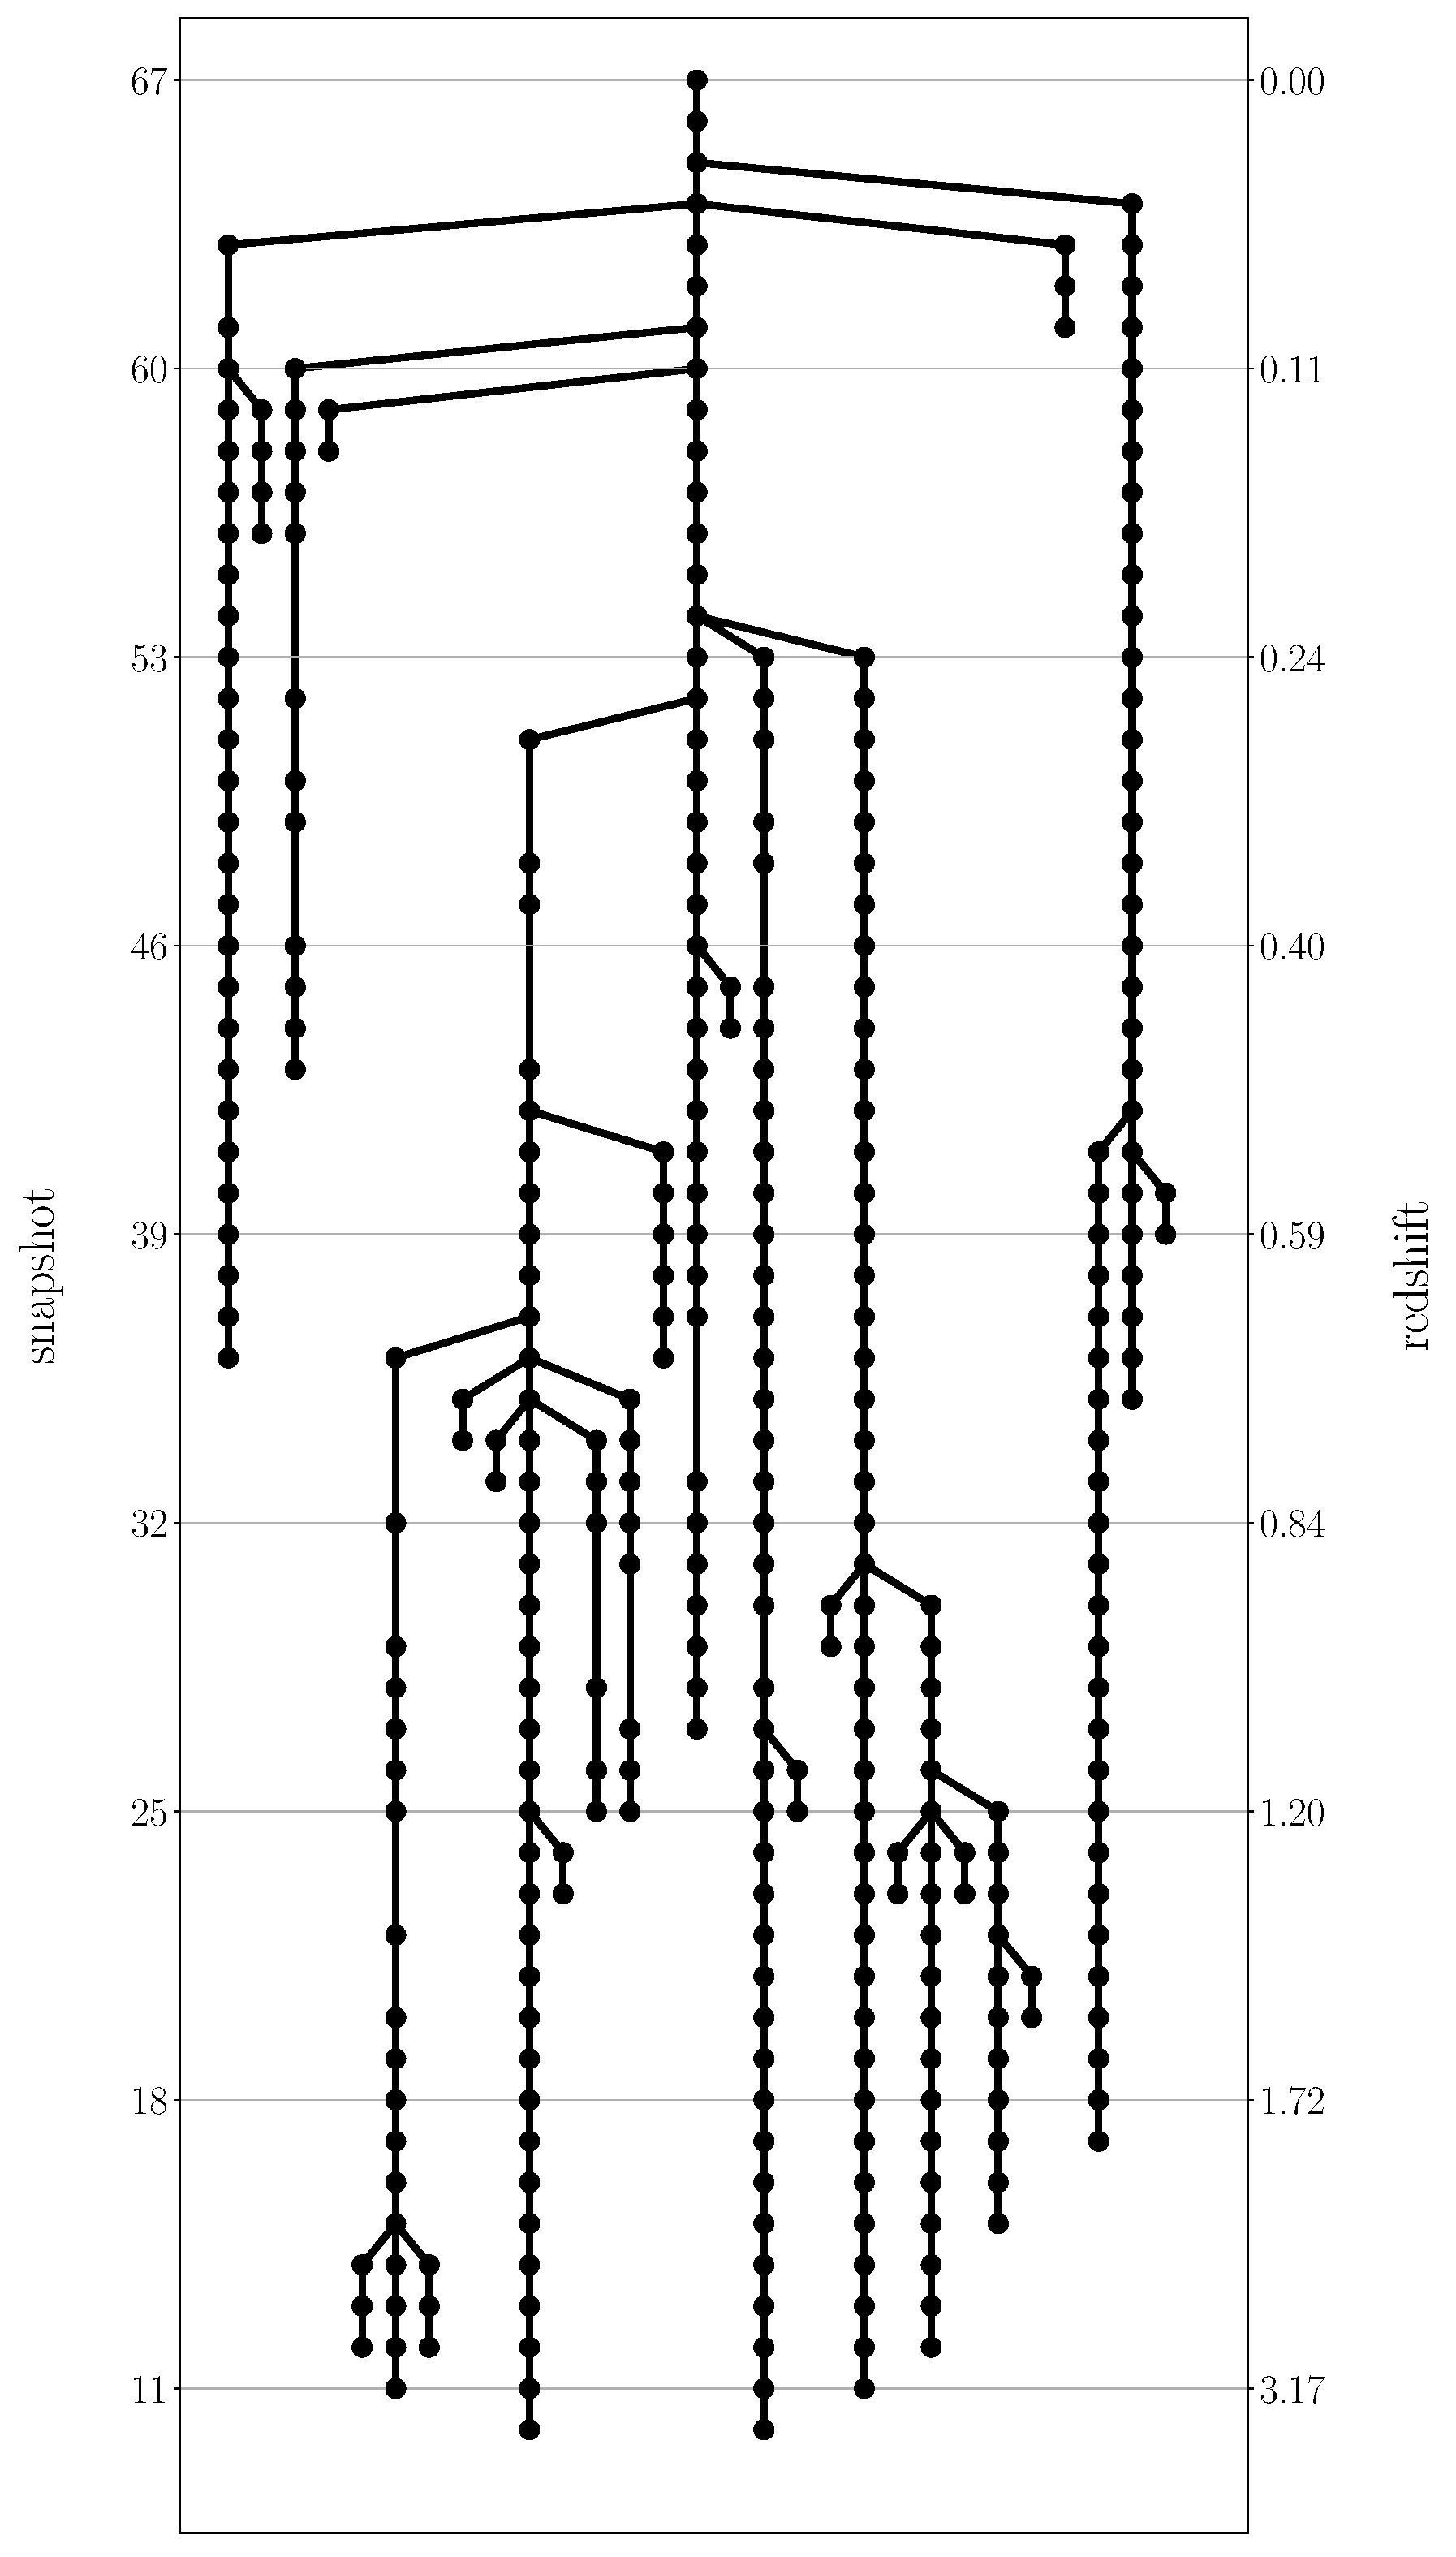
\includegraphics[width=\linewidth]{images/merger_tree_example.pdf}%
  \caption{The merger tree of a main halo at redshift zero as found by
    \texttt{ACACIA}.  This tree was extracted from a low resolution
    cosmological DMO simulation containing $64^3$ particles for
    illustrative purposes. Using higher resolutions quickly leads to
    hundreds and thousands of branches, resulting in a rather messy
    plot. On the $y$ axis, the snapshot numbers and their
    corresponding redshifts are given.  The $x$ axis has no physical
    meaning.  Each dot represents a clump identified at the given
    snapshot.  Two dots connected by a vertical line represent clumps
    that have been linked as main progenitor and main descendant.
    Diagonal lines depict merging events. In this tree, a few links
    between two dots are larger than others.  These are cases where
    clumps merge temporarily, but then re-emerge later as separate
    clumps (see the example shown in Figure~\ref{fig:jumper-demo}).
    We discuss these cases and how they are dealt with in
    Section~\ref{sect:jumpers}. }
  \label{fig:mergertree}
\end{figure} 

A straightforward method to link progenitors with descendants in two
consecutive snapshots is to trace individual particles using their
unique particle ID. All merger tree codes use this simple technique
\citep[][]{ConsistentTrees, LHaloTree, D_Trees,
  knebeImpactBaryonicPhysics2010, tweedBuildingMergerTrees2009,
  elahiClimbingHaloMerger2019a, jungEffectsLargescaleEnvironment2014,
  rodriguez-gomezMergerRateGalaxies2015} with the notable exception of
the code \texttt{JMERGE} described and tested in
\cite{SUSSING_COMPARISON}.

Linking a progenitor to a descendant means checking how many particles
of the progenitor halo or sub-halo end up in the descendant halo or
sub-halo.  Naturally, these tracer particles may end up in multiple
clumps, giving multiple descendant candidates for a progenitor.  In
such cases, the most promising descendant candidate will be called the
\emph{main descendant}.  To find a main progenitor and a main
descendant, a merit function $\mathcal{M}$ has to be defined, which is
to be maximised or minimised, depending on its definition.  An
overview of the merit functions that are used in other merger tree
algorithms is given in Table~1 of \cite{SUSSING_COMPARISON}.  The
merit function used in our implementation is given in
Equation~\ref{eq:merit}.

Sometimes, unfortunately, linking progenitors to descendants is not as
straightforward as described so far. We now discuss two circumstances
where special care must be taken to define robust links between
different snapshots: fragmentation events and temporary merger events.

%Because galaxies form inside the potential well dark matter haloes,
%knowledge of how many merging events a halo underwent during its
%lifetime is crucial for accurate mock galaxy catalogues.  After a
%merging event, the galaxy of the smaller halo that has been
%``swallowed up'' by a bigger one has no reason to simply vanish
%without a trace.  The ``swallowed up'' halo might become a sub-halo,
%or, if it is small enough or after some time, it might not be
%detectable as substructure in the simulation any more.  Galaxies of
%haloes that dissolve in this manner are referred to as ``\emph{orphan
%galaxies}'' \citep[e.g.][]{subfind}.

\begin{figure}
  \centering
  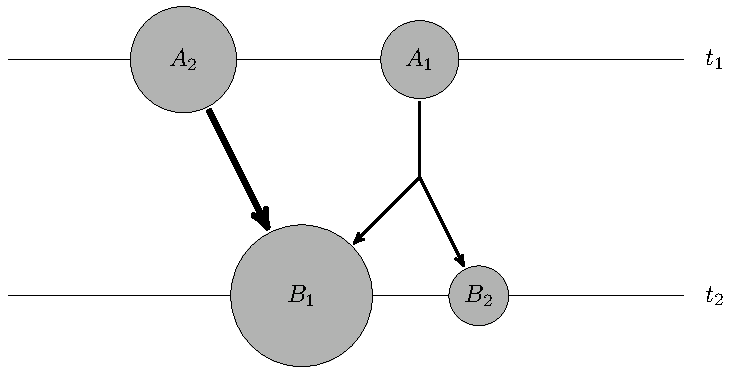
\includegraphics[width=.9\linewidth]{./images/tikz/fracture.pdf}
  \caption{Illustration of a progenitor $A_1$ at time $t_1$ which is
    partially merged into a descendant $B_1$ at time $t_2 > t_1$, but
    some other part $B_2$ isn't.  Because $A_1$ is not the main
    progenitor of $B_1$, by assigning its descendant only according to
    the merit function \eqref{eq:merit} would not pass on its
    formation history to $B_2$, but treat it as newly formed.  The
    size of the circles represents the haloes' masses, the $x$-axis
    has no physical meaning.  }
  \label{fig:fracture}
\end{figure}

\subsection{Fragmentation Events}
\label{sect:frag}

%See https://arxiv.org/pdf/2010.03567.pdf Fig. 34
In our current approach, each progenitor can have only one
descendant\footnote{Note that \cite{springelSimulatingCosmicStructure2021a}
proposed another approach that allows explicitly fragmentation
events to be included in the merger tree analysis.}. We therefore need
to pick only one descendant within a possibly large ranked list of
descendant candidates, that all contain particles coming from the
progenitor.

Normally, this choice is performed according to the ranking provided
by the merit function, where the main descendant is ranked number 1.
Problems arise for example when the progenitor $A_1$ is not the main
progenitor of its main descendant $B_1$, but also has fragmented into
another viable descendant candidate $B_2$.  This situation is
schematically shown in Figure~\ref{fig:fracture}.

Relying only on the merit function \eqref{eq:merit}, progenitor $A_1$
will seem to have merged with $A_2$, the direct progenitor of $B_1$,
in order to form $B_1$.  The other fragment, $B_2$, will be treated as
a newly formed clump and the entire formation history of $B_2$ would
be lost. In order to preserve this history, we choose to prioritize the 
link from $A_1$ to $B_2$ over of merging progenitor $A_1$ into $B_1$.


It is simpler to deal with this case directly in the algorithm
than via the merit function. The resulting logic can be summarized as
follows: If $A_1$ is not the main progenitor of its main descendant
$B_2$, then we don't merge it into $B_2$ but we link it instead with
the first secondary descendants that considers $A_1$ as its
main progenitor.

%This way, we give priority to $A_1$ for being a progenitor to some descendant which is
%not its main descendant over merging it into its main descendant.  In
%other words: being a main progenitor will have more weight on the tree
%building scheme than being a main descendant.

\subsection{Temporary Merger Events}
\label{sect:jumpers}

\begin{figure}[!htbp]
    {
%        \renewcommand{\arraystretch}{0.1}
        \setlength\tabcolsep{0em}
    	\centering	
    	\begin{tabular}{|p{5.3cm}p{5.3cm}p{5.3cm}|}
    		\hline
    		%		 
    		{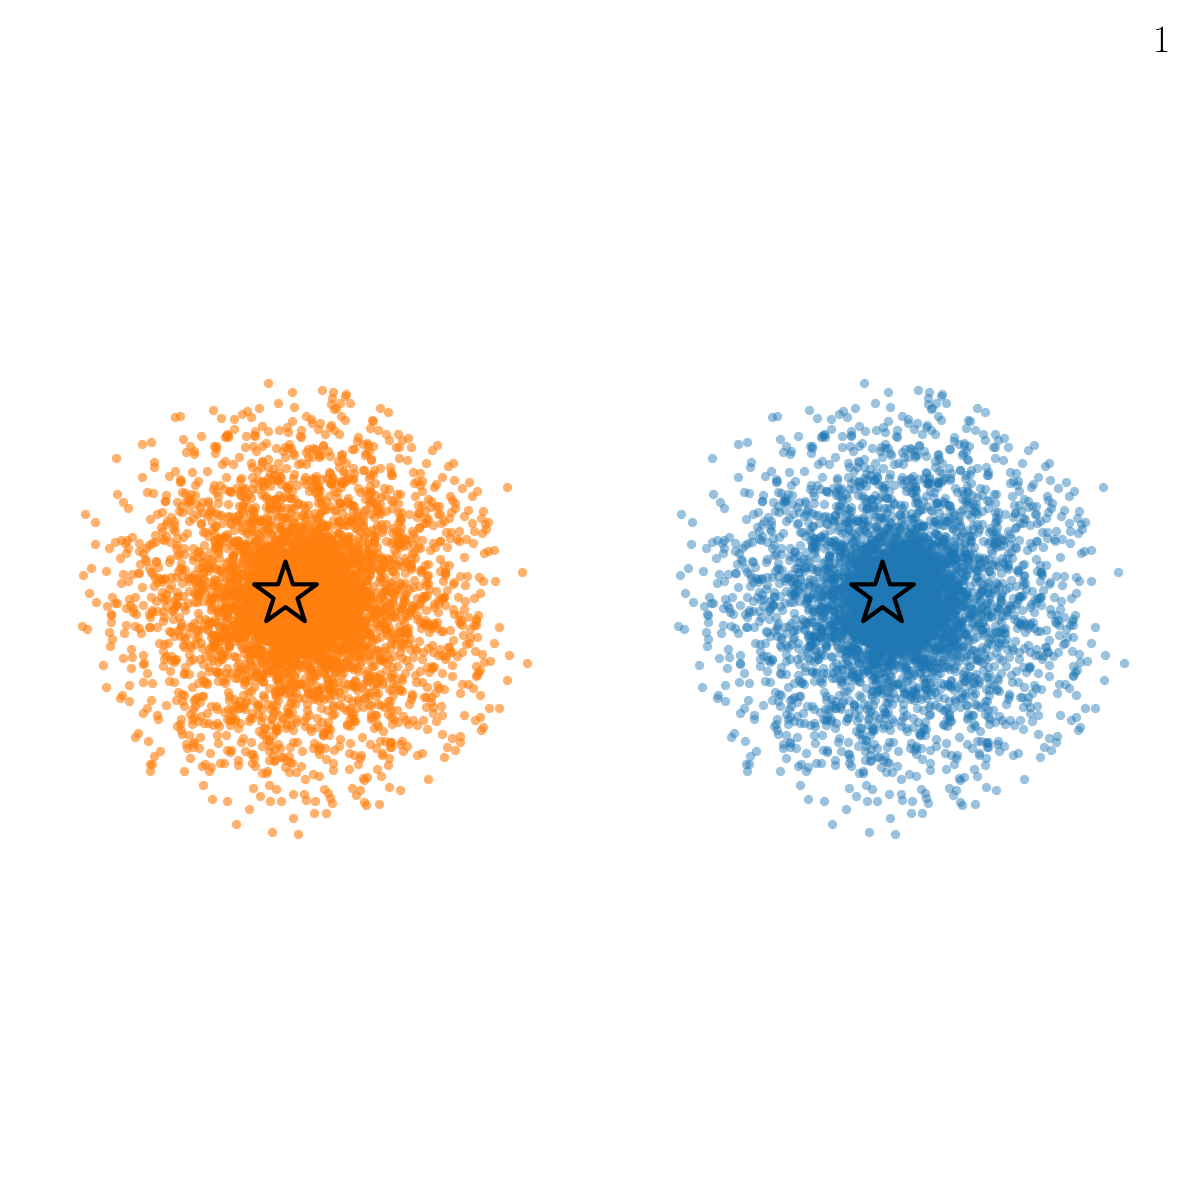
\includegraphics[width = 5.3cm]{images/jumper-demo/particleplot_00001.png}}	& 
    		{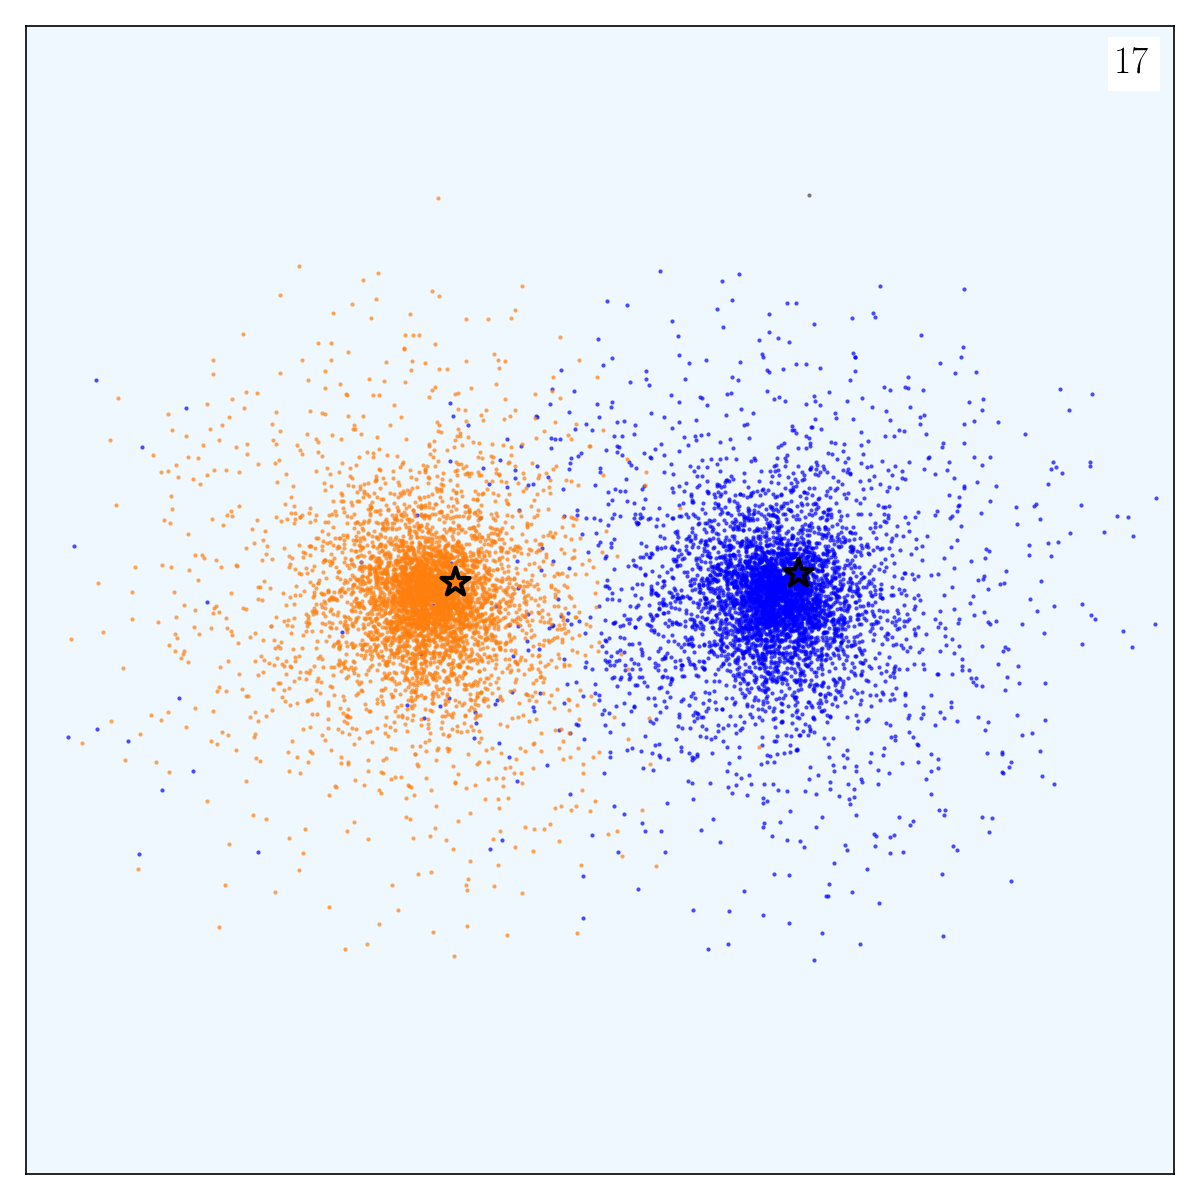
\includegraphics[width = 5.3cm]{images/jumper-demo/particleplot_00017.png}}	& 
    		{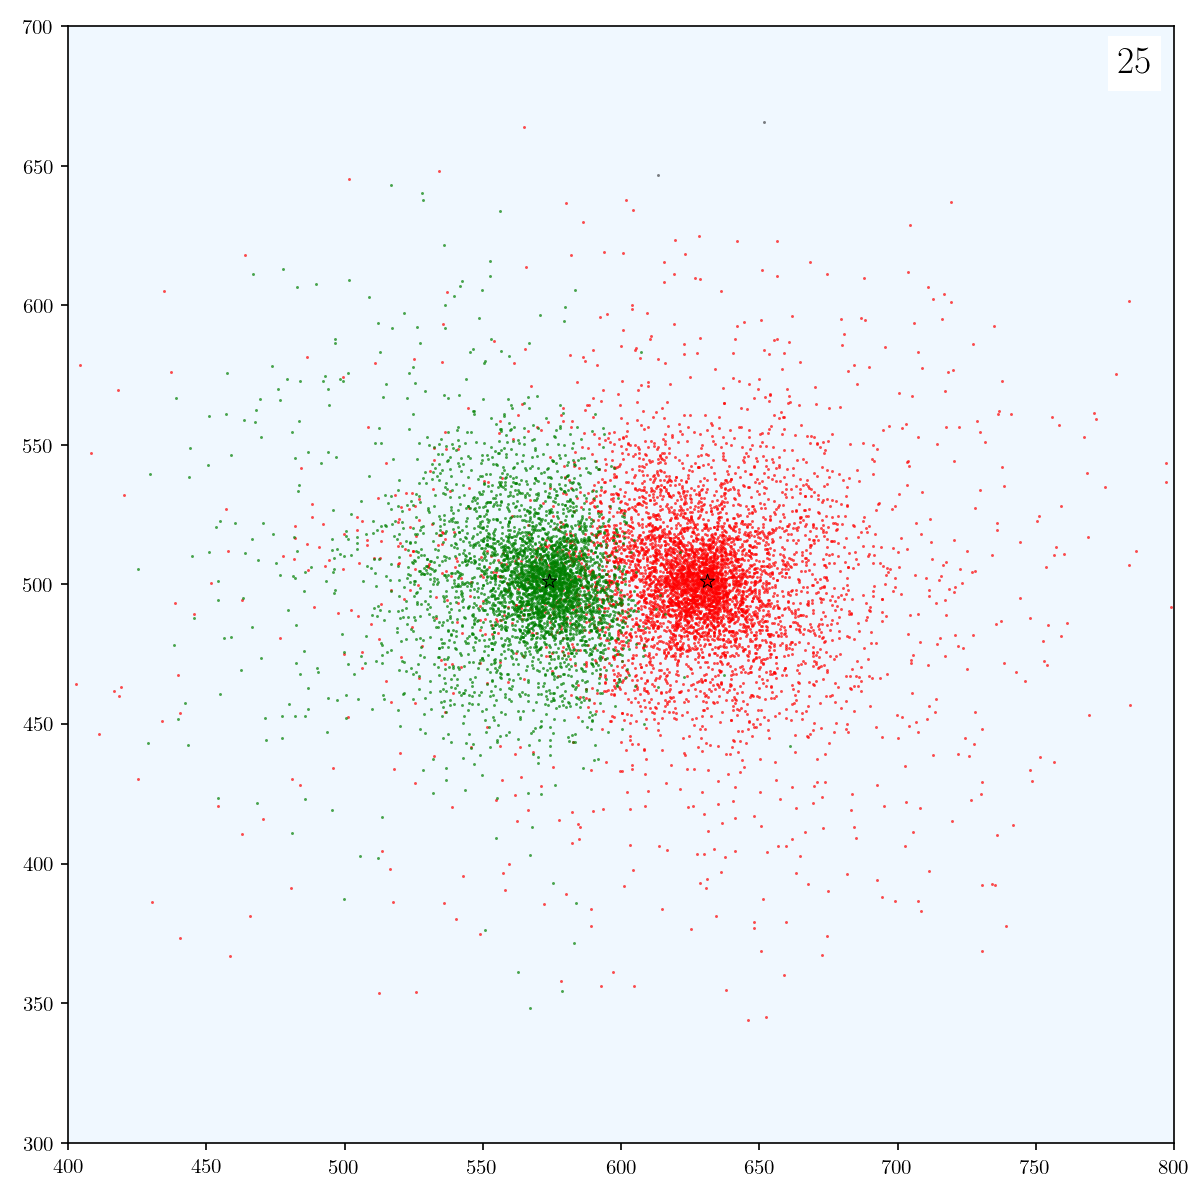
\includegraphics[width = 5.3cm]{images/jumper-demo/particleplot_00025.png}}  \\[-0.5em]
    		%
    		%
    		{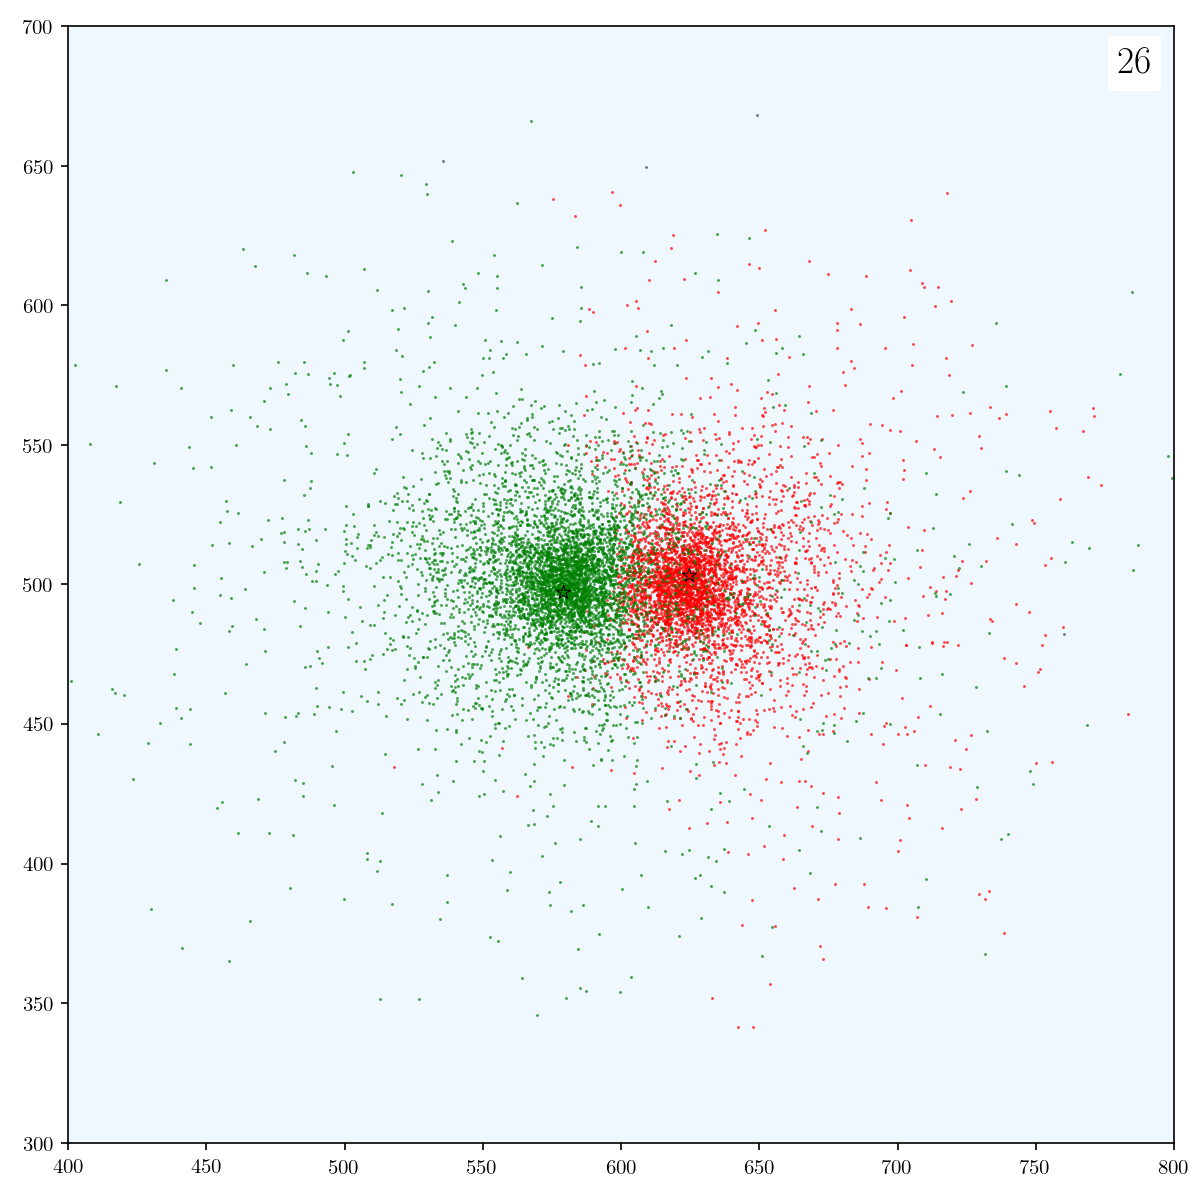
\includegraphics[width = 5.3cm]{images/jumper-demo/particleplot_00026.png}}	& 
    		{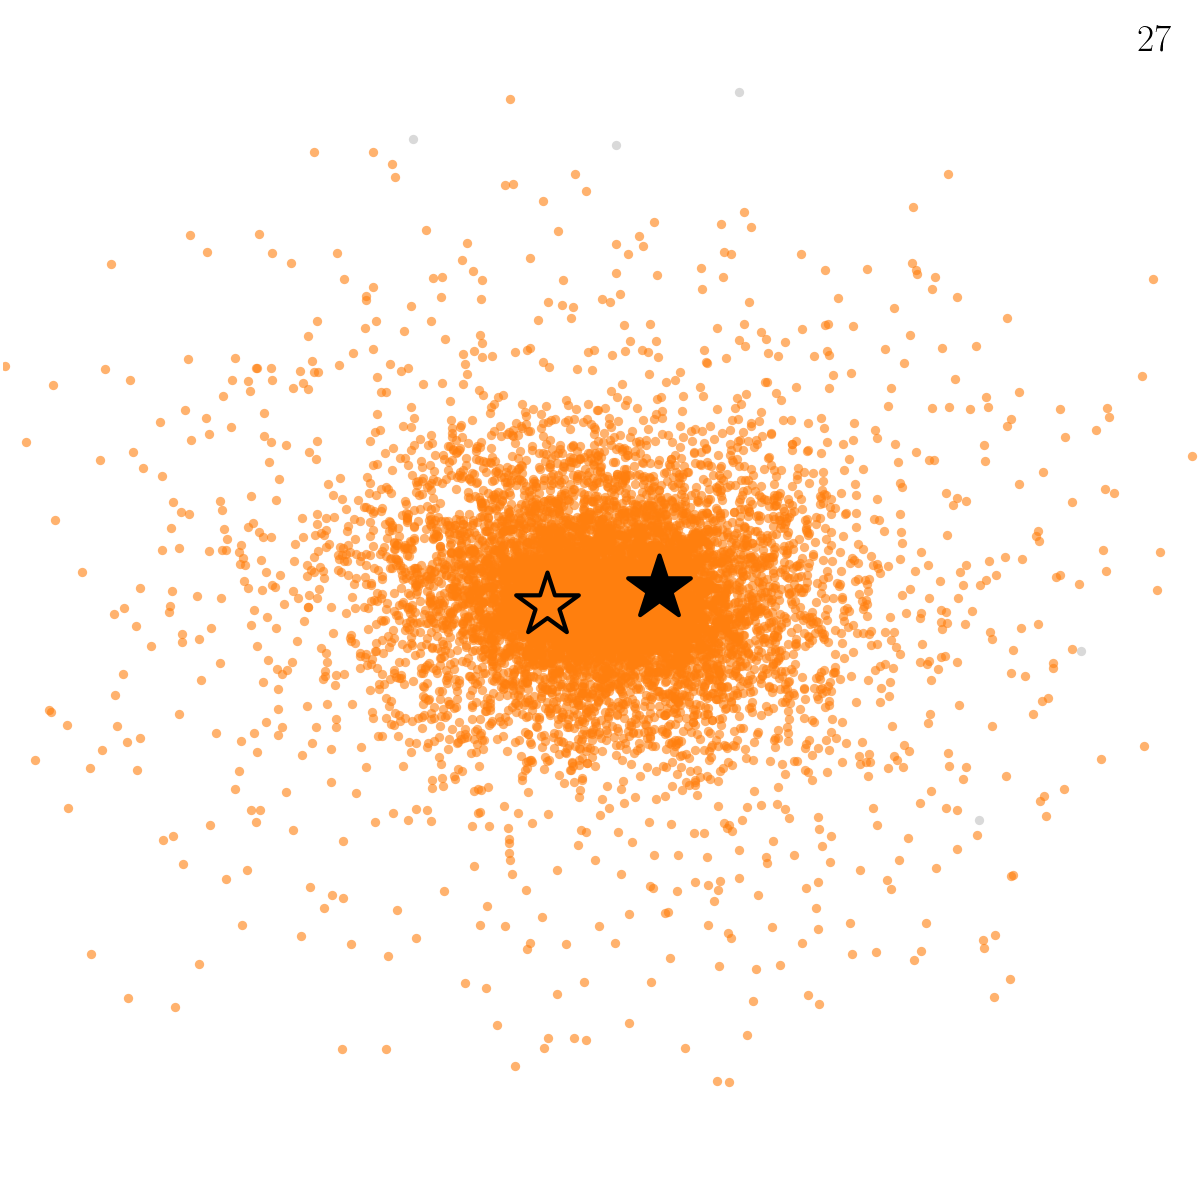
\includegraphics[width = 5.3cm]{images/jumper-demo/particleplot_00027.png}}	& 
            {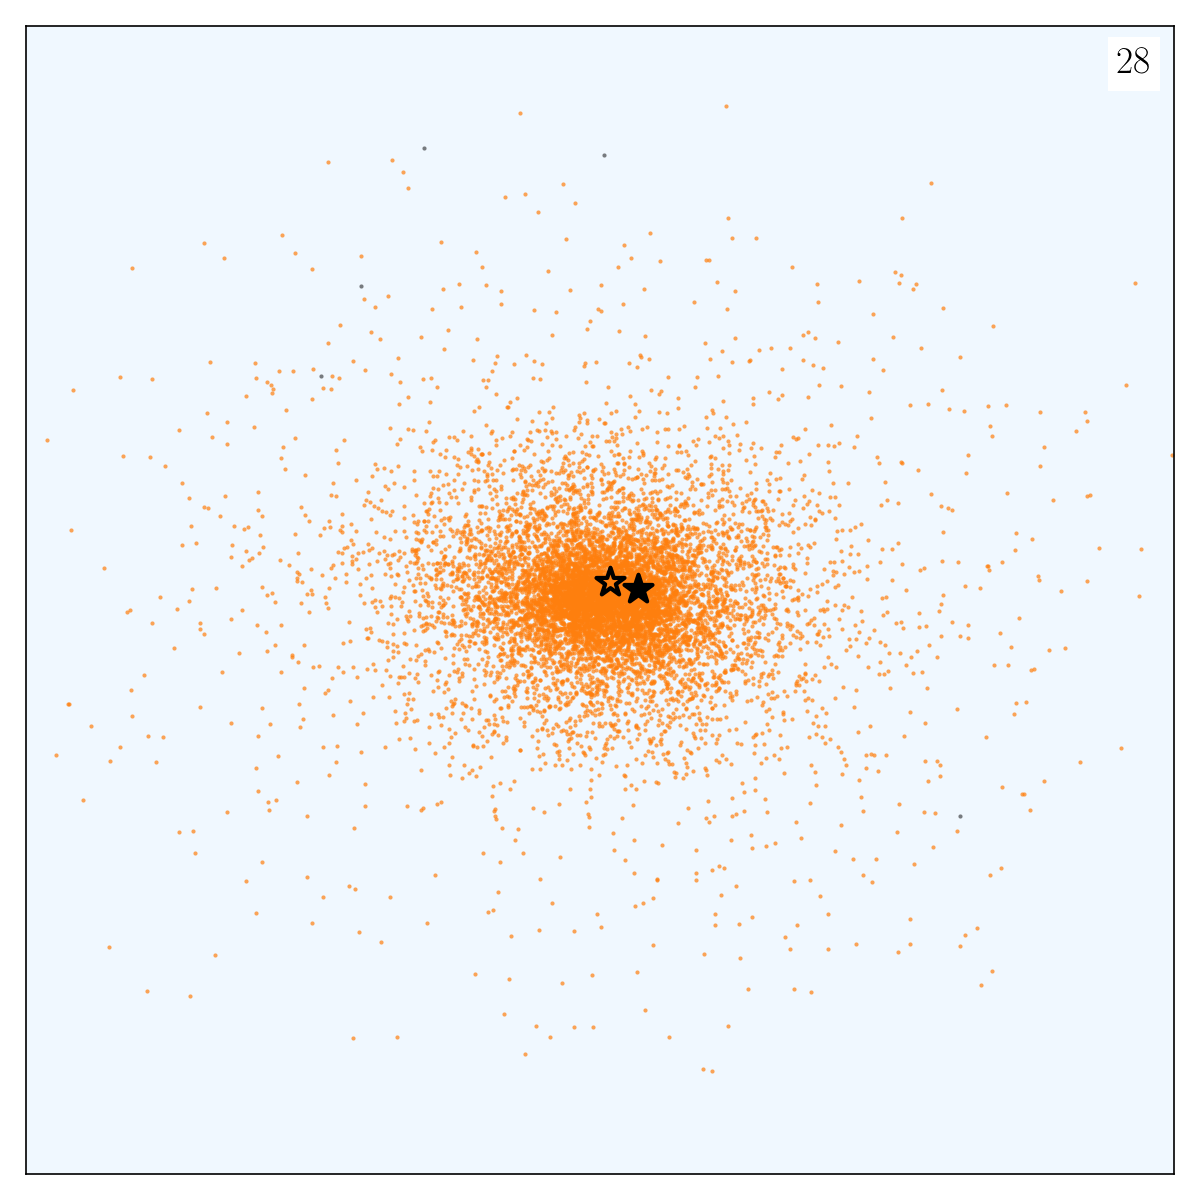
\includegraphics[width = 5.3cm]{images/jumper-demo/particleplot_00028.png}}	\\[-0.5em] 
    		%
            %
            {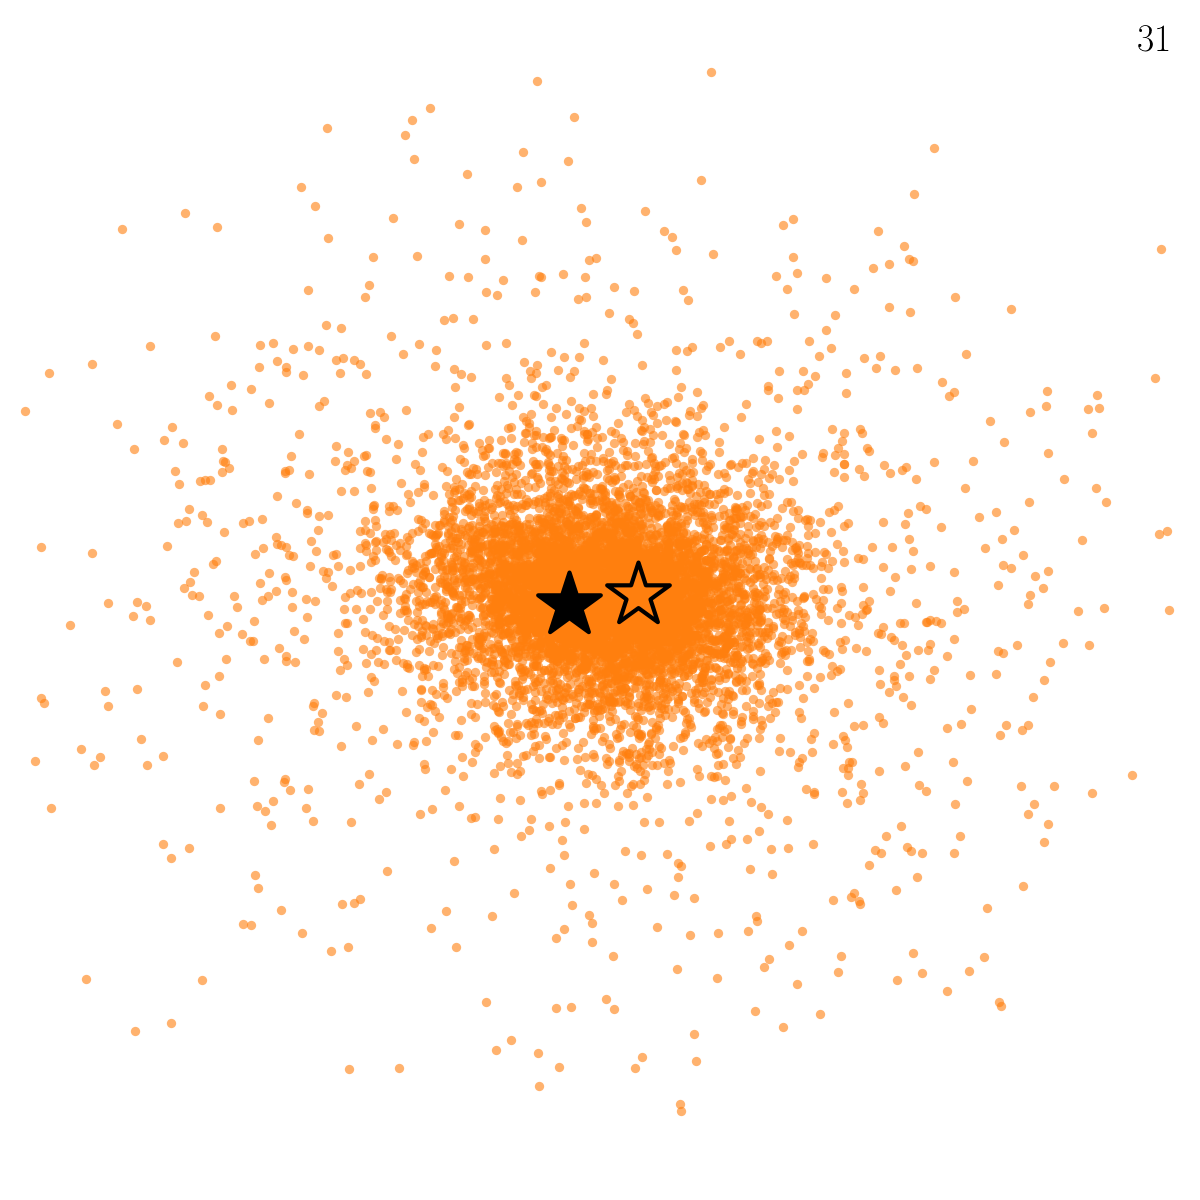
\includegraphics[width = 5.3cm]{images/jumper-demo/particleplot_00031.png}}    &
            {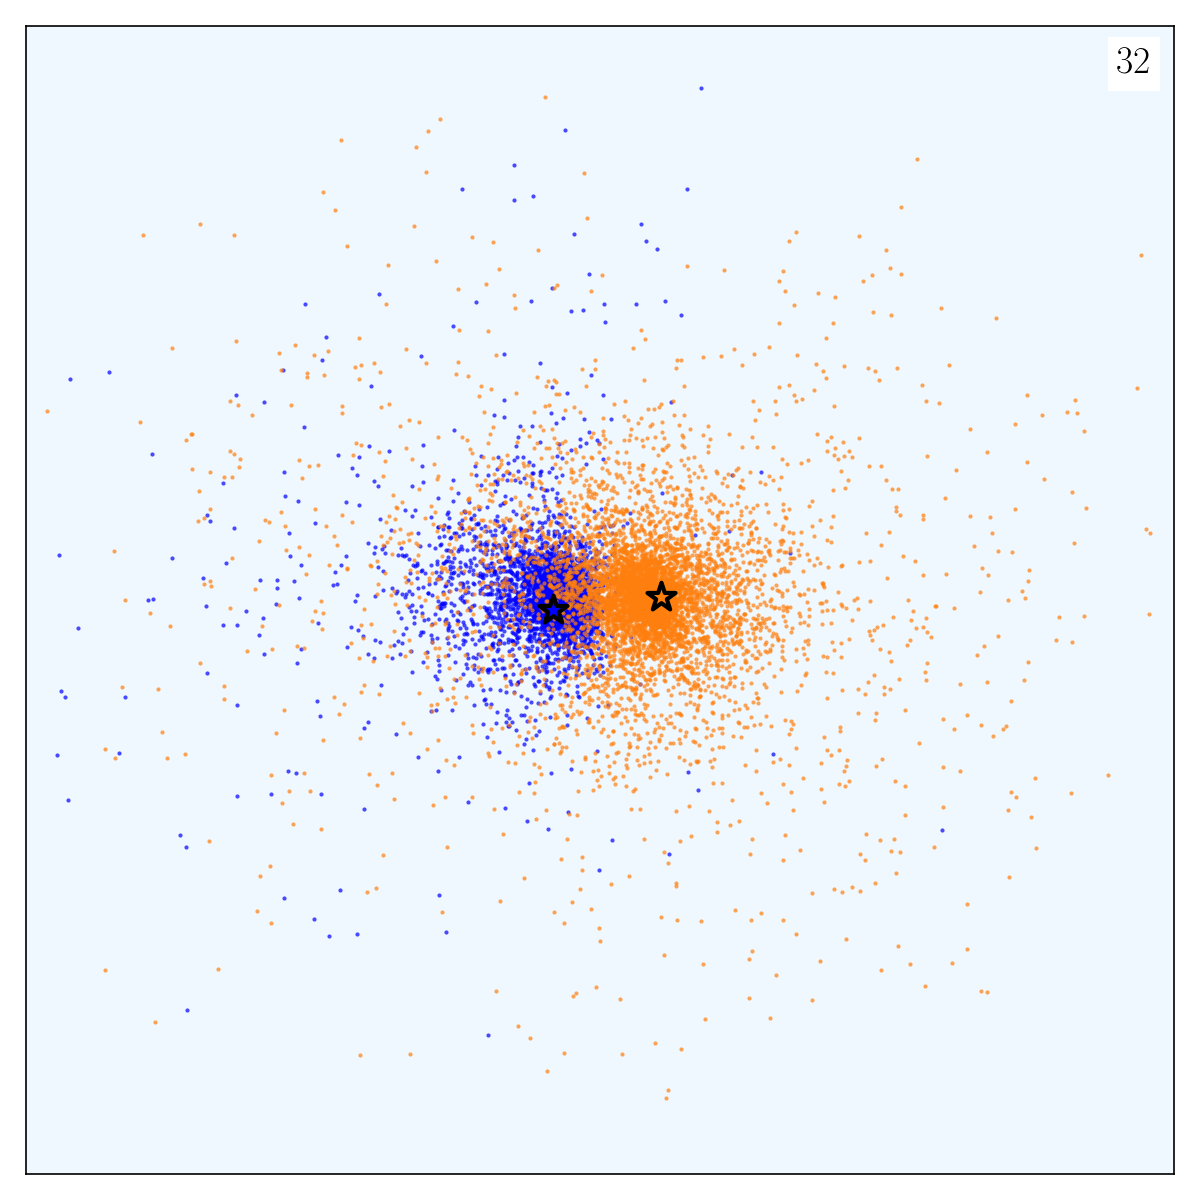
\includegraphics[width = 5.3cm]{images/jumper-demo/particleplot_00032.png}} 	&
            {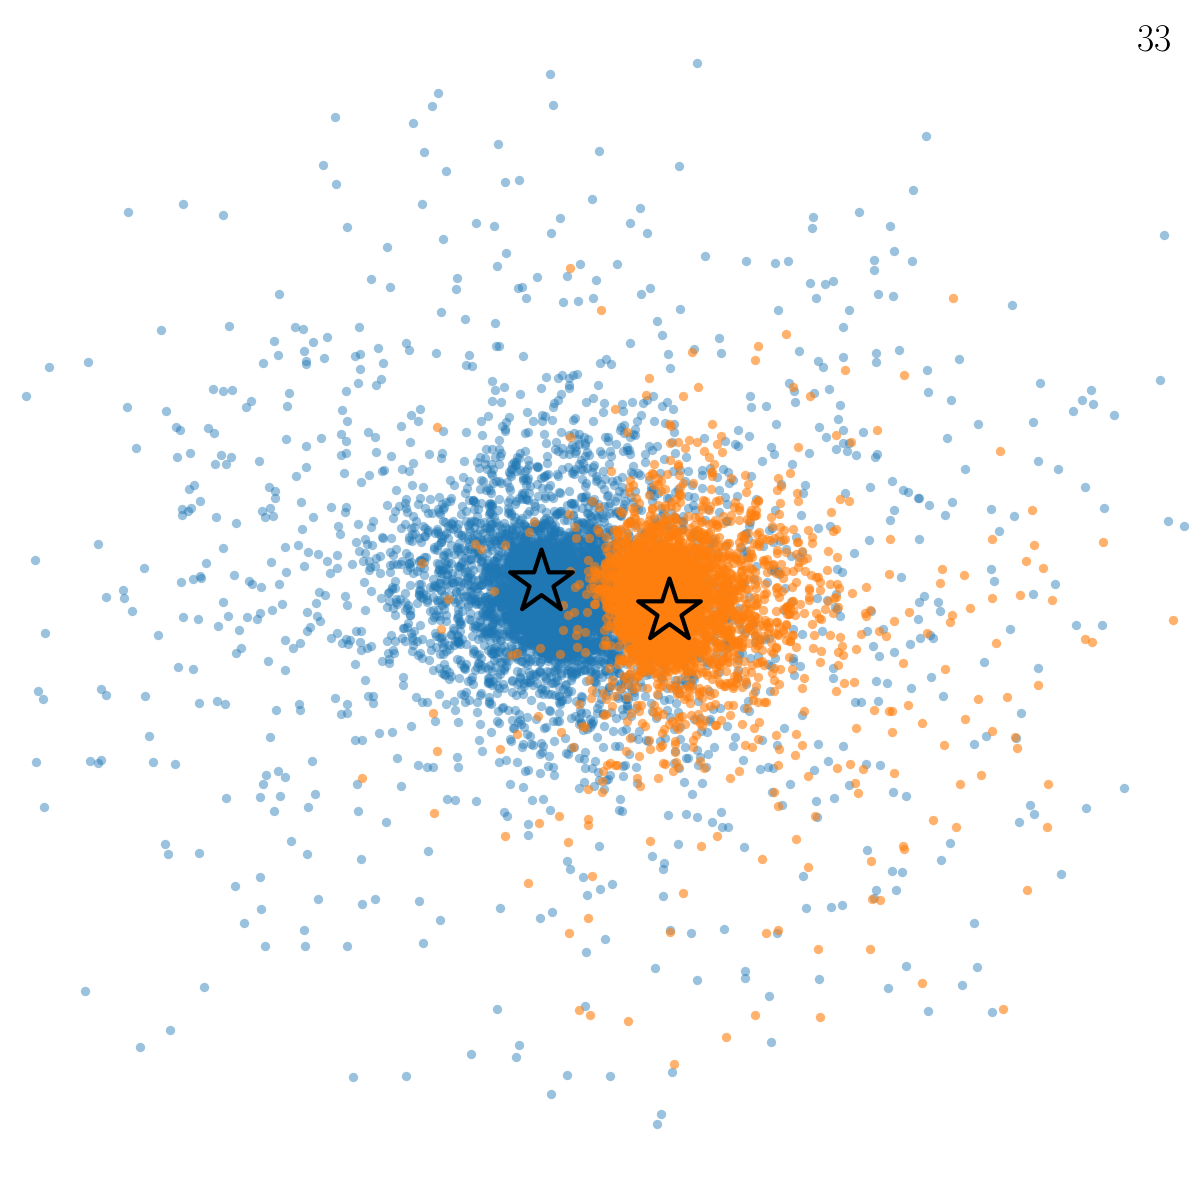
\includegraphics[width = 5.3cm]{images/jumper-demo/particleplot_00033.png}} 	\\[-0.5em]
    		%
            %
            {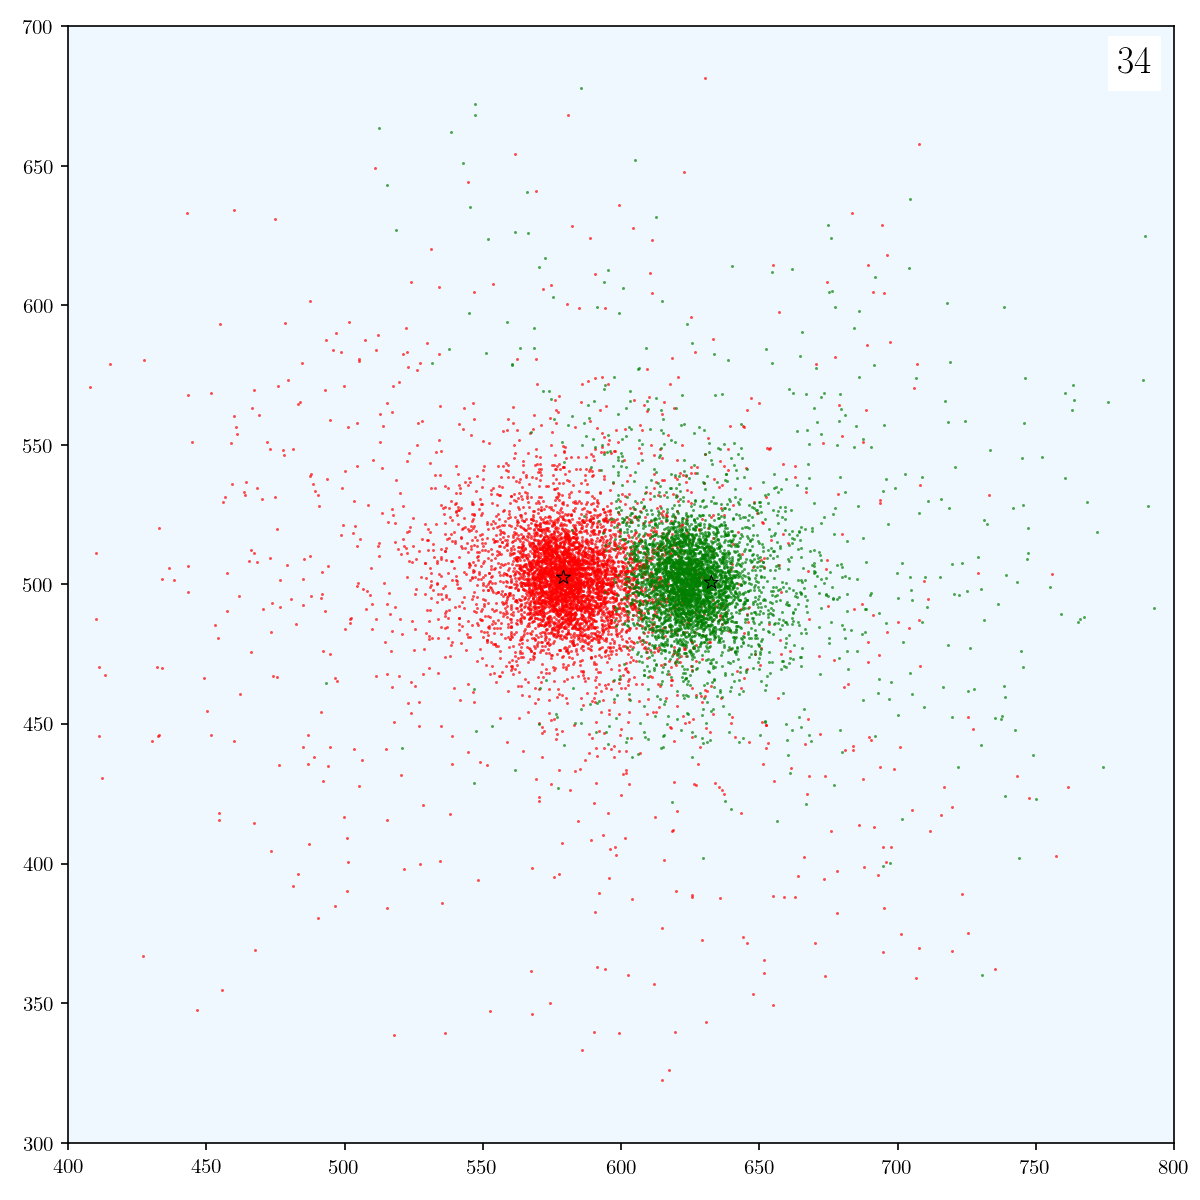
\includegraphics[width = 5.3cm]{images/jumper-demo/particleplot_00034.png}} 	& 
    		{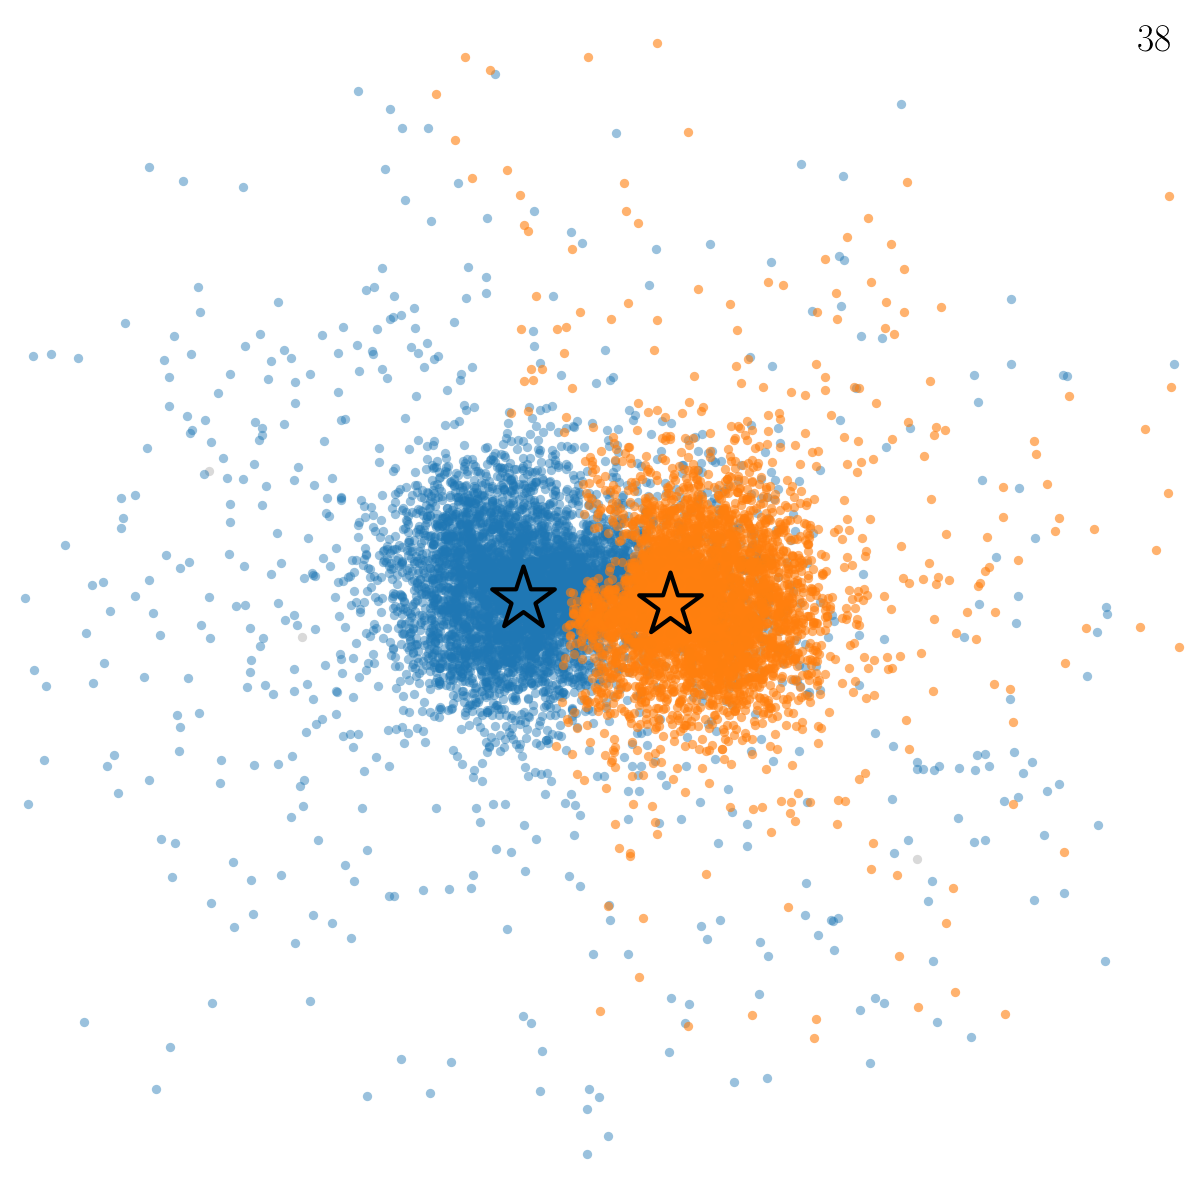
\includegraphics[width = 5.3cm]{images/jumper-demo/particleplot_00038.png}}	& 
            {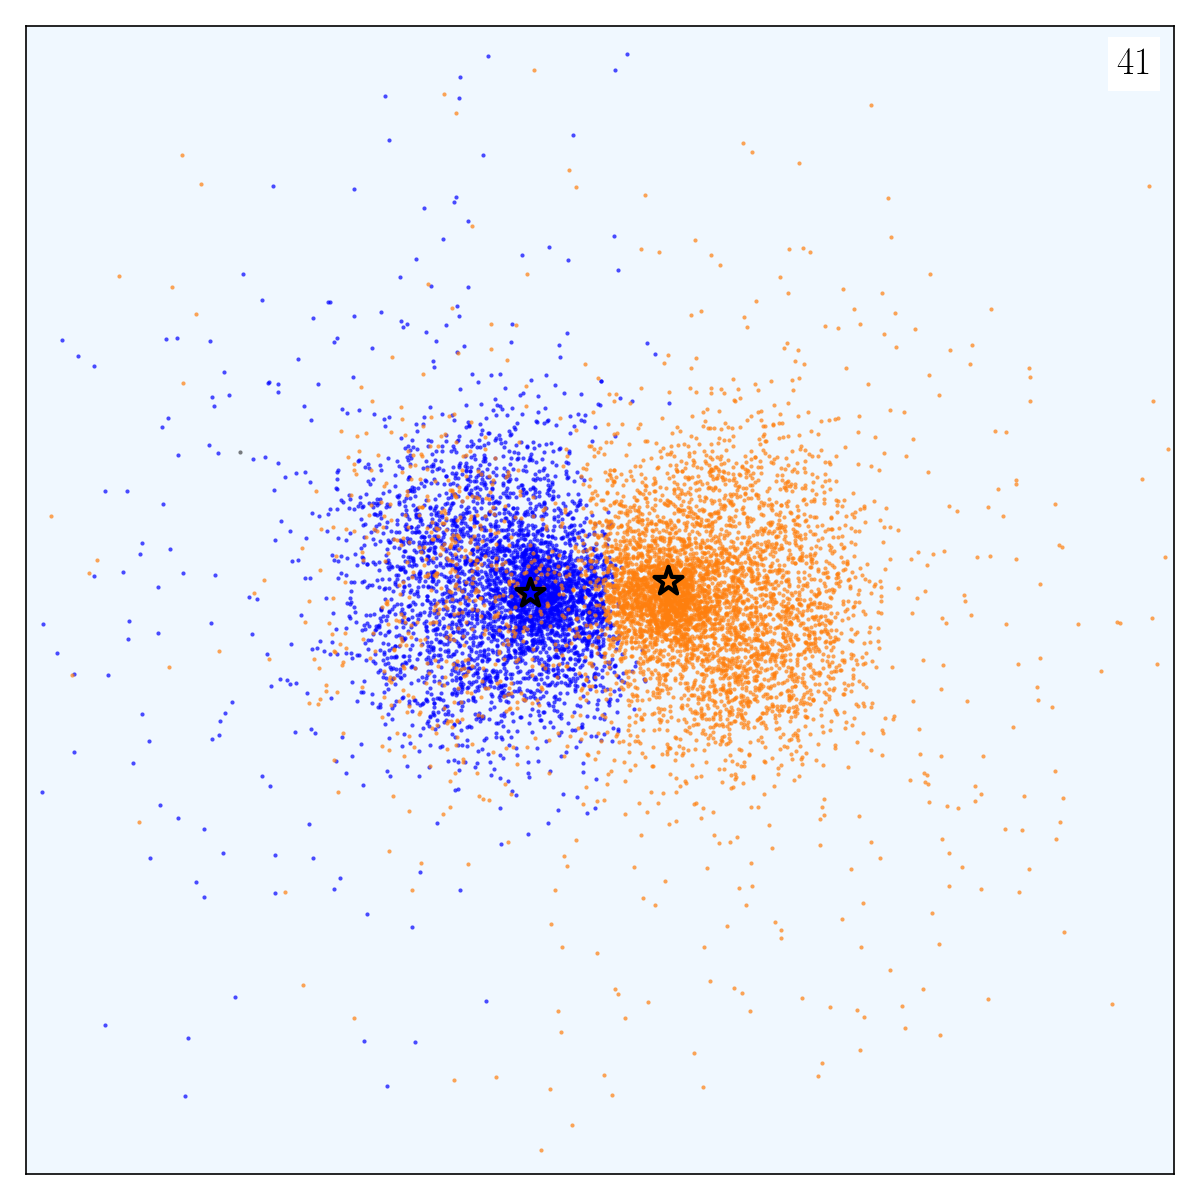
\includegraphics[width = 5.3cm]{images/jumper-demo/particleplot_00041.png}} 	\\%[-0.5em]
    		%
            %
%            {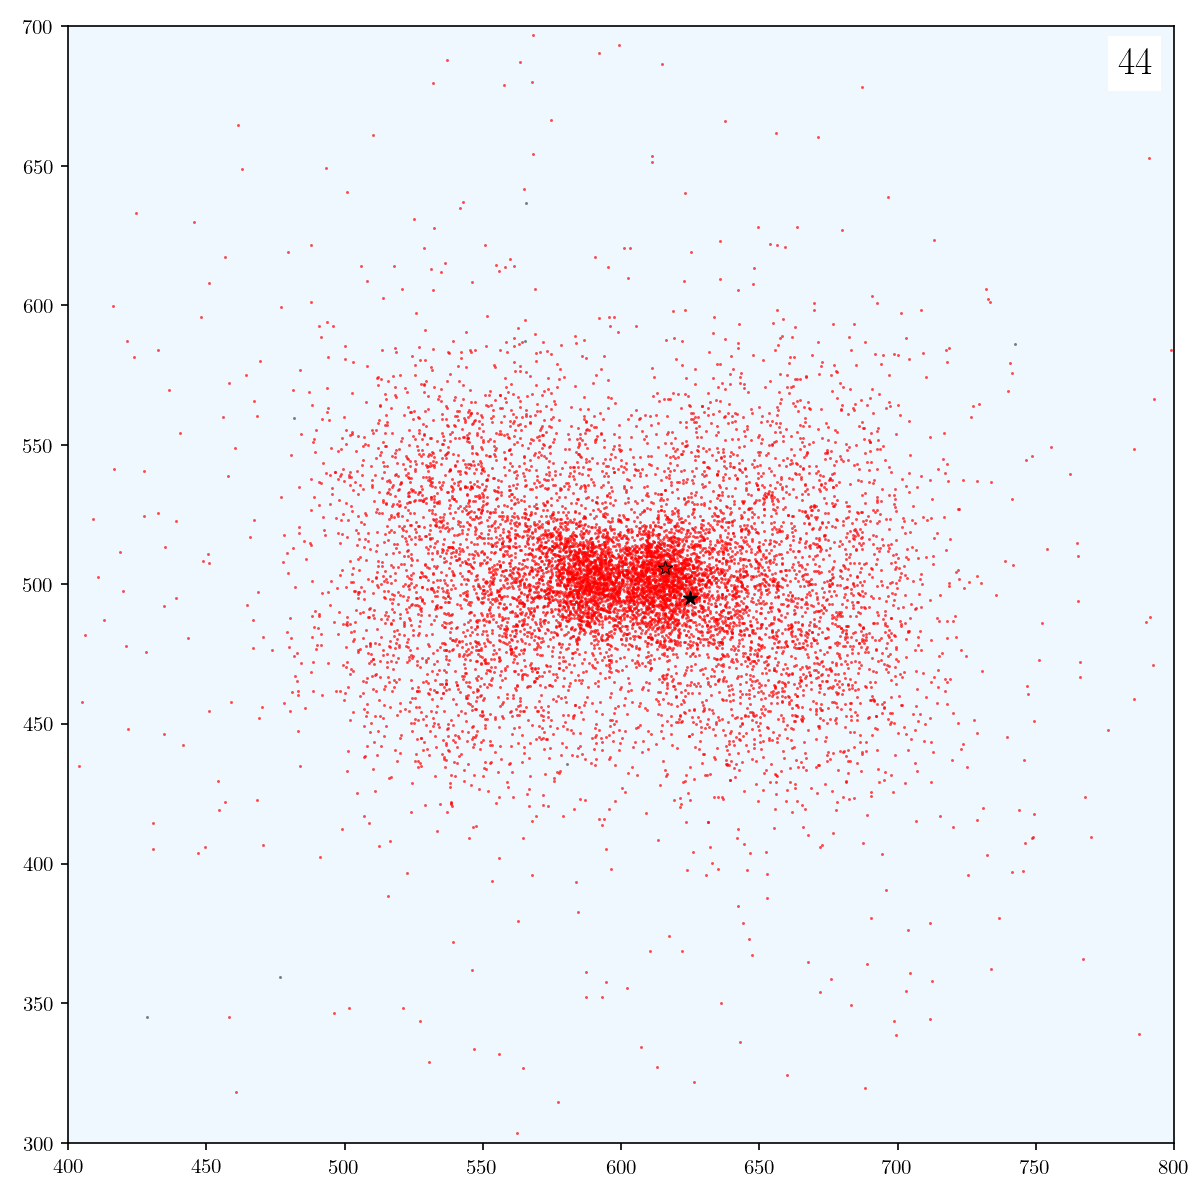
\includegraphics[width = 5.3cm]{images/jumper-demo/particleplot_00044.png}} 	& 
%    		{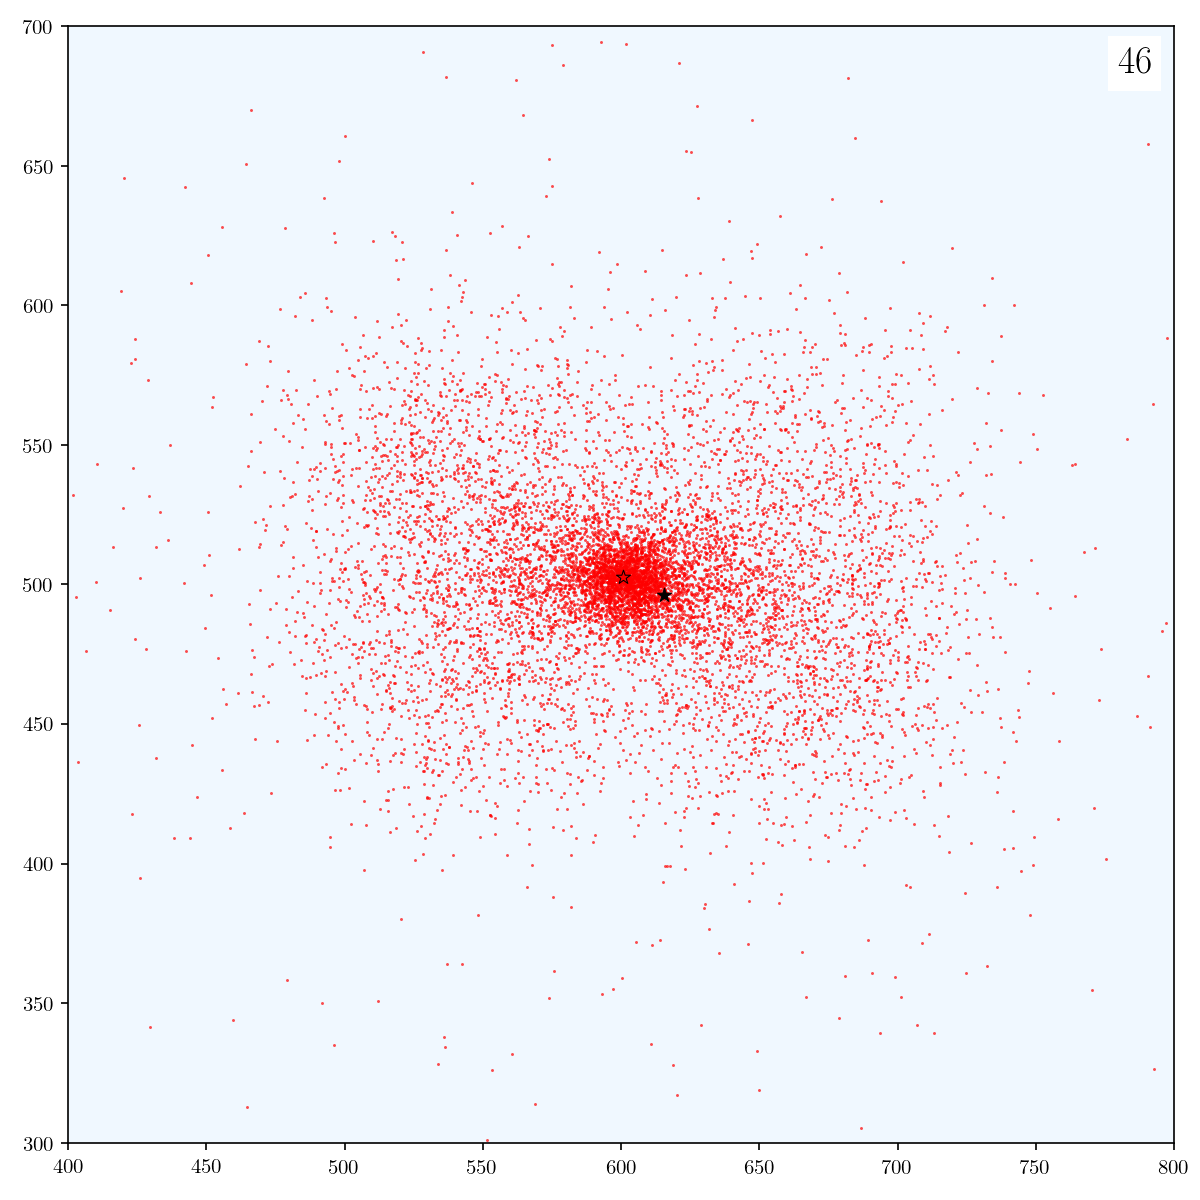
\includegraphics[width = 5.3cm]{images/jumper-demo/particleplot_00046.png}}	& 
%            {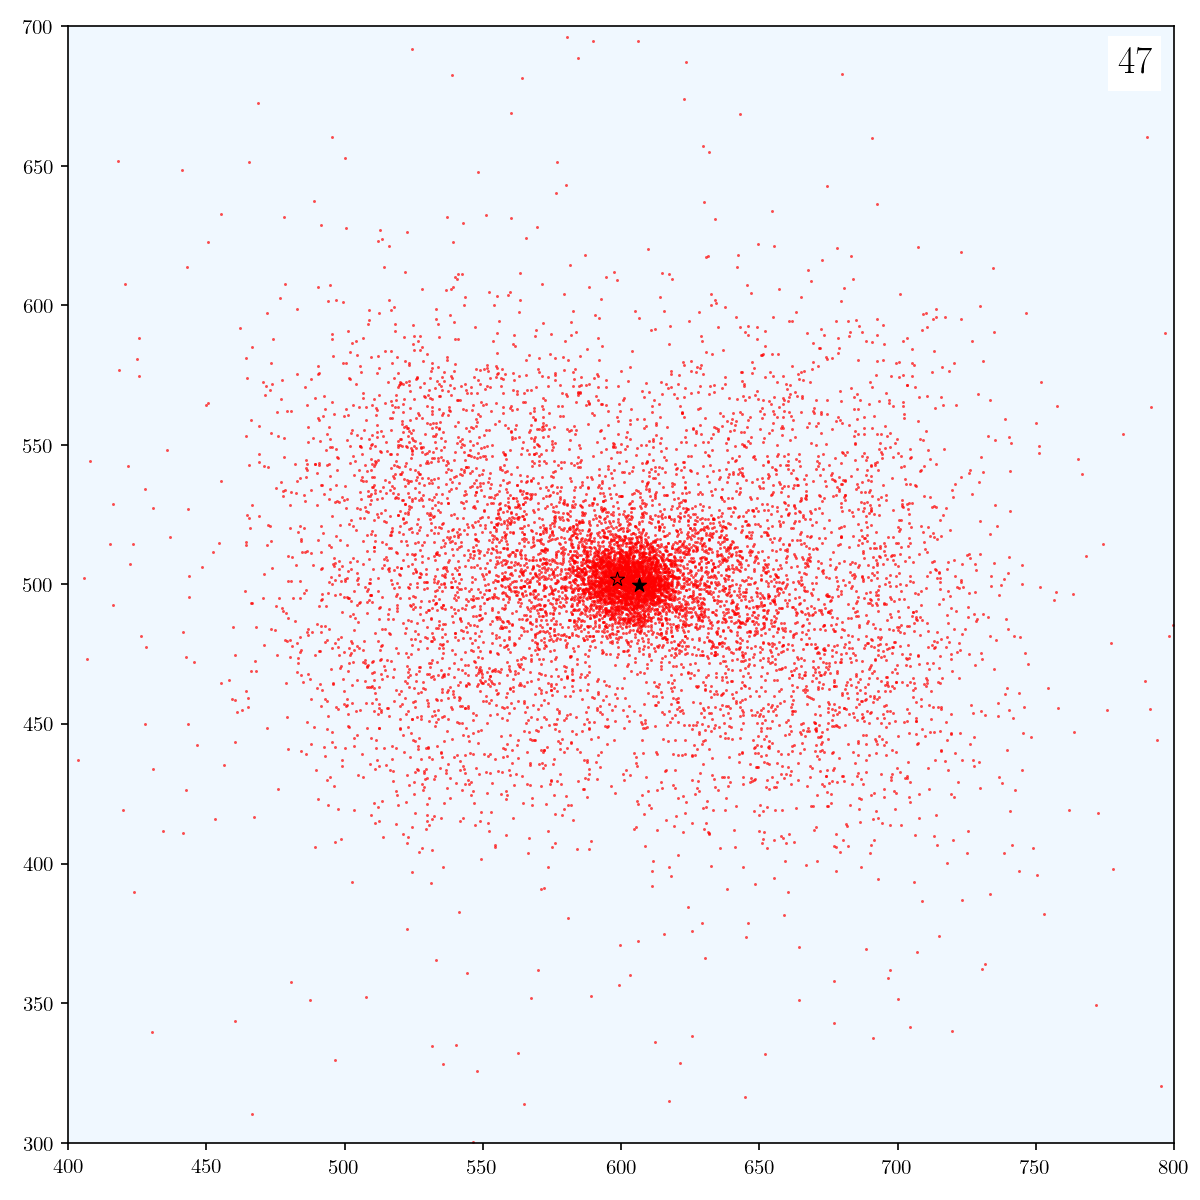
\includegraphics[width = 5.3cm]{images/jumper-demo/particleplot_00047.png}} 	& 
%            {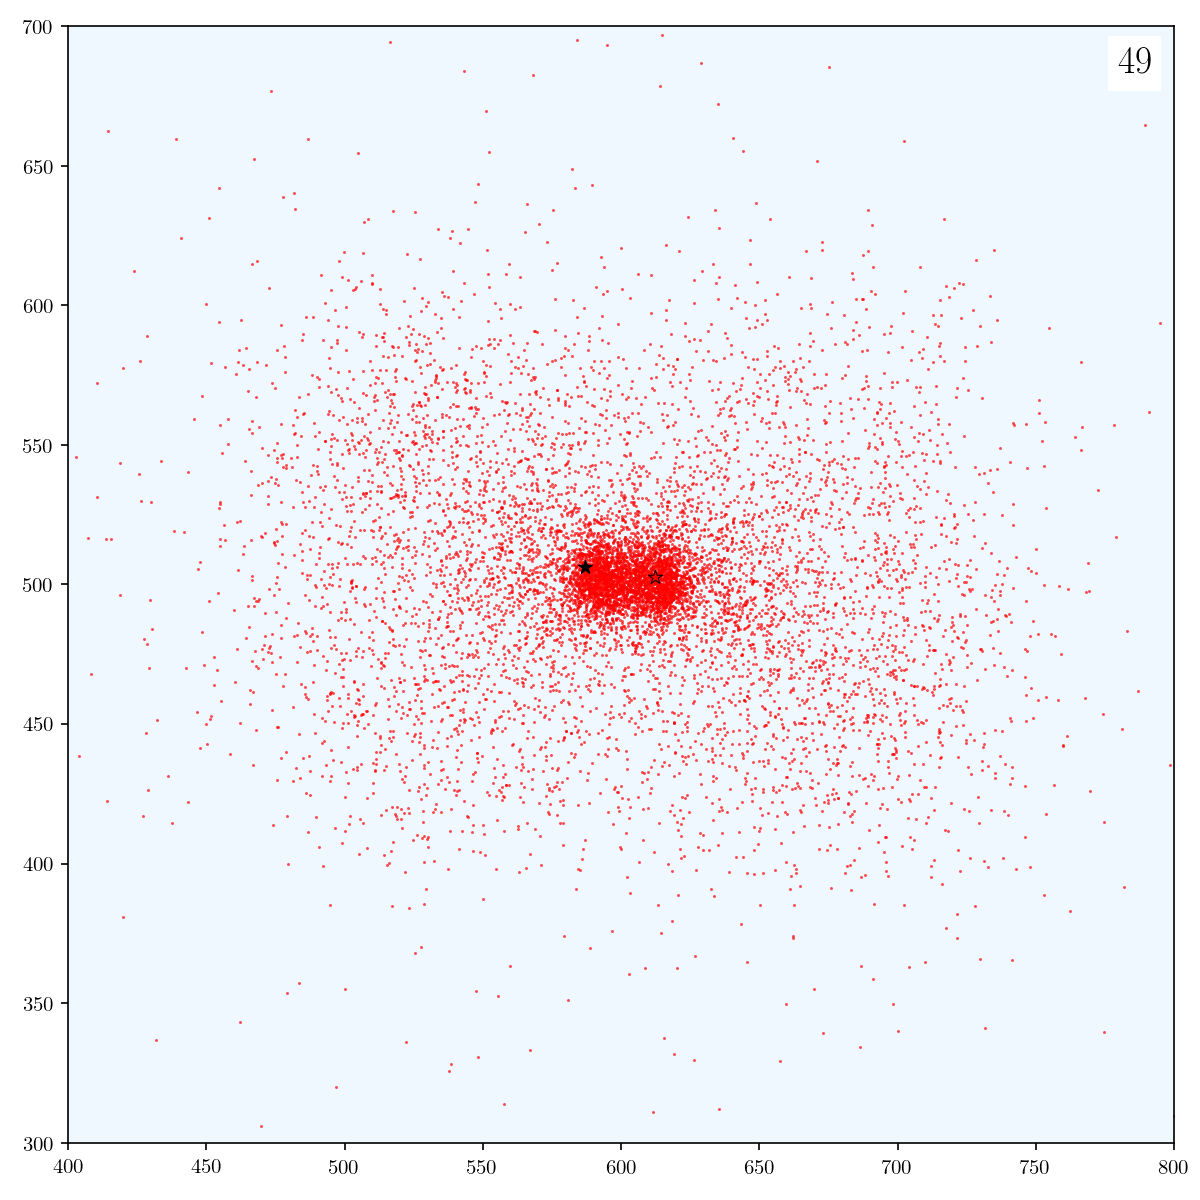
\includegraphics[width = 5.3cm]{images/jumper-demo/particleplot_00049.png}}  \\
        	\hline
    	\end{tabular}
    }
	\caption{\label{fig:jumper-demo} 
        Illustration of how haloes can seemingly merge into another one and re-appear a few snapshots later.
        The green and red particles are two initially distinct haloes that pass through each other.
        The galaxies assigned to them are marked by a star with the same colour as the particles.
        Black stars mark orphan galaxies, which have lost their unique host halo.
        The number in the upper right corner of each plot is the snapshot number that is depicted.
        In snapshots 27-31, the halo-finding algorithm didn't identify both haloes as distinct objects.
        However by tracking the red halo's orphan galaxy, it was possible to link the halo in snapshot 32 all the way back to snapshot 26.\\        
        The simulation was created using \texttt{DICE} \parencite{DICE}.
        Both haloes are identical with mass of $5\cdot 10^{10}\msol$, each containing 5000 particles and following a NFW mass profile.
        The plotted region corresponds to $400$ kpc on each side.
        }
\end{figure}




























































%\begin{sidewaysfigure}[!htbp]
%	{\renewcommand{\arraystretch}{0.1}
%		
%	\subfloat[The results of \phewon\ and \simple\ unbinding of the \ds-dataset: All particles, halo-namegiver particles only and subclumps particles only.]{
%		\begin{tabular}{|p{1cm} c c c|}
%			\hline
%			&&&\\[1em]
%													&
%			\textbf{All particles} 					&
%			\textbf{Halo-namegiver particles only} 	&
%			\textbf{Subhalo particles only} 		\\[1em]
%			%
%			%
%			\begin{sideways}{\hspace{3cm} \phewon}\end{sideways} \hspace*{-1em}%		 
%			& {\includegraphics[width = .28\textwidth]{images/dice-sub/dice-sub-plot-halo1-phew.png}} \hspace*{-1em}%
%			 & {\includegraphics[width = .28\textwidth]{images/dice-sub/dice-sub-halo-only-phew.png}} \hspace*{-1em}% 
%			 &{\includegraphics[width = .28\textwidth]{images/dice-sub/dice-sub-plot-subclumps-phew.png}} \\
%			%
%			%
%			\begin{sideways}{ \hspace{3cm}\simple\ unbinding }\end{sideways}	 \hspace*{-1em}			 &
%			{\includegraphics[width = .28\textwidth]{images/dice-sub/dice-sub-plot-halo1-nosaddle.png}} \hspace*{-1em}&
%			{\includegraphics[width = .28\textwidth]{images/dice-sub/dice-sub-halo-only-nosaddle.png}} \hspace*{-1em}&
%			{\includegraphics[width = .28\textwidth]{images/dice-sub/dice-sub-plot-subclumps-nosaddle.png}} \\
%			\hline
%		\end{tabular}
%		\label{fig:dice_sub_results_a}
%		}
%	}
%	\phantomcaption
%\end{sidewaysfigure}
%%=================================================
%%=================================================
%%=================================================
%\begin{sidewaysfigure}[!htbp]\ContinuedFloat
%	\footnotesize
%	{\renewcommand{\arraystretch}{0.1}
%	\subfloat[The results of \neigh\ and \iter\ unbinding of the \ds-dataset: All particles, halo-namegiver particles only and subclumps particles only.]{
%		\begin{tabular}{|p{1cm} c c c|}
%			\hline
%			&&&\\[1em]
%													&
%			\textbf{All particles} 					&
%			\textbf{Halo-namegiver particles only} 	&
%			\textbf{Subhalo particles only}			\\[1em]
%			%
%			%
%			\begin{sideways}{ \hspace{3cm}\neigh\ unbinding }\end{sideways}		\hspace*{-1em}		 &		
%			{\includegraphics[width = .28\textwidth]{images/dice-sub/dice-sub-plot-halo1-saddle.png}}\hspace*{-1em} &
%			{\includegraphics[width = .28\textwidth]{images/dice-sub/dice-sub-halo-only-saddle.png}}\hspace*{-1em} &
%			{\includegraphics[width = .28\textwidth]{images/dice-sub/dice-sub-plot-subclumps-saddle.png}} \\
%	%		%
%	%		%
%			\begin{sideways}{\hspace{3cm} \iter\ unbinding }\end{sideways}		\hspace*{-1em}		 &		
%			{\includegraphics[width = .28\textwidth]{images/dice-sub/dice-sub-plot-halo1-iter.png}} \hspace*{-1em}&
%			{\includegraphics[width = .28\textwidth]{images/dice-sub/dice-sub-halo-only-iter.png}} \hspace*{-1em}&
%			{\includegraphics[width = .28\textwidth]{images/dice-sub/dice-sub-plot-subclumps-iter.png}} \\
%			%
%			%
%			\hline
%		\end{tabular}
%		\label{fig:dice_sub_results_b}
%		}
%	}
%	\caption{
%	The results of different unbinding methods on the \dt-dataset.
%	}
%	\label{fig:dice_sub_results}
%\end{sidewaysfigure}
%
%

When a sub-halo travels towards the core of its parent halo, it will
merge with the central clump and disappear from the sub-halo lists.  It
can however re-emerge at a later snapshot and will be added back
to the list as a newly born halo. Such a scenario is shown in
Figure~\ref{fig:jumper-demo}.  Indeed, when this occurs, the merger
tree code will deem the sub-halo to have merged into the main halo, and
will likely find no progenitor for the re-emerged sub-halo, thus
treating it as newly formed.

This is a problematic case because we lose track of the growth history
of the sub-halo, regardless of its size, and massive clumps may be
found to just appear out of nowhere in the simulation.  This is a well
known problem for configuration-space halo finders
\citep{onionsSubhaloesGoingNotts2012}, and phase-space halo finders
like \texttt{ROCKSTAR} \citep{behrooziRockstarPhaseSpaceTemporal2013}
have been developed precisely to alleviate this issue.  While they
typically perform better than configuration-space halo finders,
\cite{SUSSING_COMPARISON} found that phase-space halo finders aren't
infallible in recovering all such missing haloes, and strongly
recommend checking for links between progenitors and descendants in
non-consecutive snapshots as well.

As our merger tree code works on the fly, future snapshots will not be
available at the time of the merger tree analysis, so it will be
necessary to check for progenitors of a descendant across multiple
snapshots.  This can be achieved by keeping track of the most bound
particles of each clump when it is merged into some other clump.
These tracer particles are also used to track {\it orphan galaxies}.
\footnote{In the context of SAM, orphan galaxies are galaxies born at
the center of dark matter haloes that merged later into bigger haloes
and eventually dissolved due to over-merging. As a consequence, these
galaxies don't have a parent halo or sub-halo anymore.}  For this
reason, we call these tracer particles ``orphan particles'', and
progenitor-descendant links over non-adjacent snapshots ``jumpers''.

These jumper links between different haloes widely separated in time
are less reliable than proper links between progenitors and
descendants from adjacent snapshots.  As we will discuss
in Section~\ref{chap:testing-nmb}, the quality of the merger trees
increases with the number of tracer particles used.  Using jumpers
corresponds to using only one tracer particle over a large time interval,
much larger than the one between two adjacent snapshots.

For this reason, priority is given to direct progenitor candidates in
adjacent snapshots.  Only if no direct progenitor candidates have been
found for some descendant, then progenitor candidates from
non-adjacent snapshots are searched for.  Because these progenitors
from non-adjacent snapshots are only tracked by one single particle,
we don't use the merit function to rank them.  Instead, we find the
orphan particle within the descendant clump which is the most tightly
bound.

In conclusion, although not ideal, using jumpers remains a necessity
to track these temporary merger events.  As a bonus, it allows us to
track orphan galaxies as will be discussed in
Section~\ref{chap:mock_catalogues}.





%============================================
\section{Details Of Our New Algorithm}\label{chap:my_code}
%============================================

\begin{figure*}
	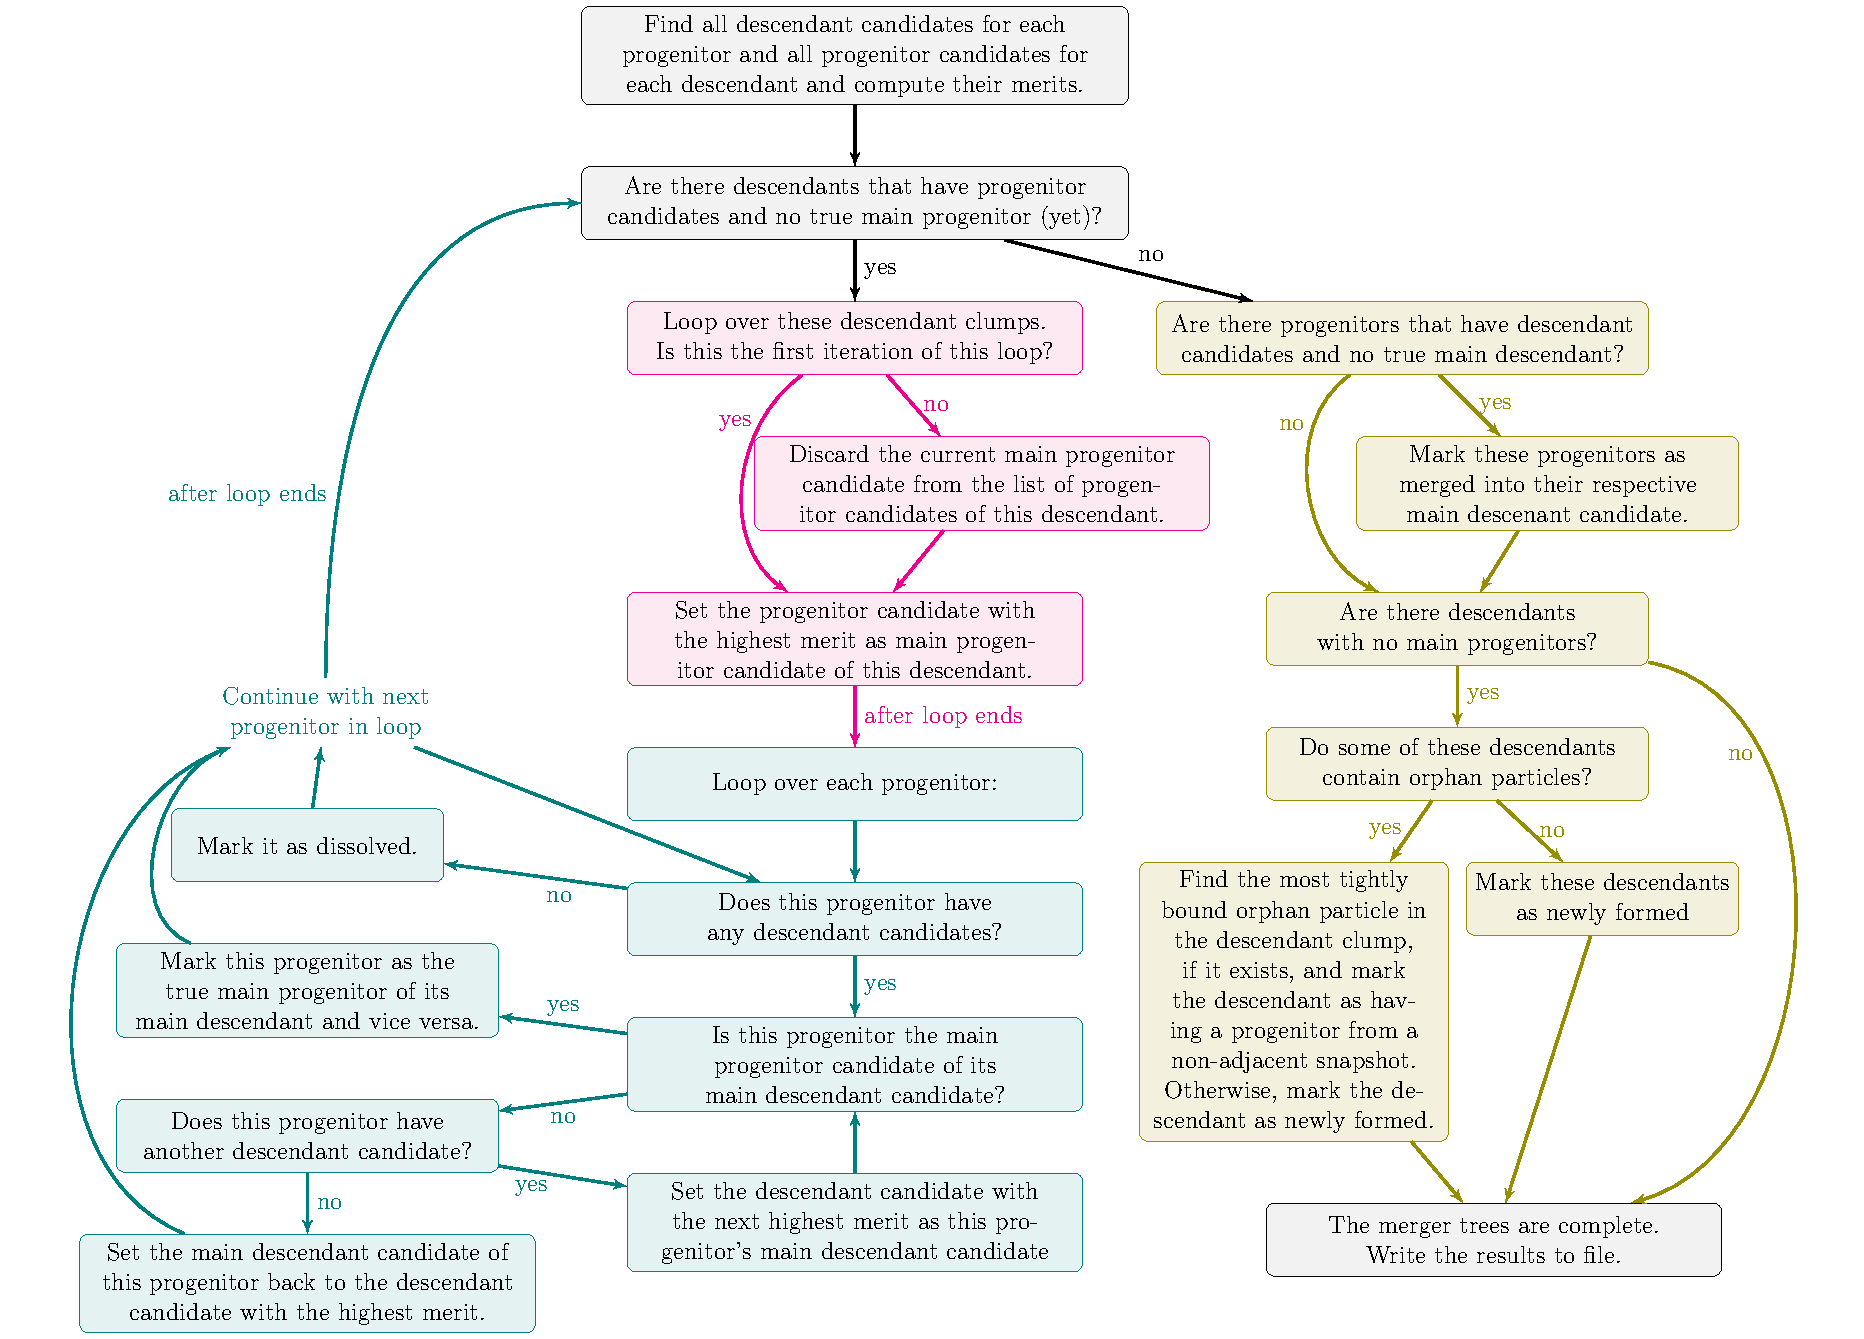
\includegraphics[width=\textwidth]{./images/tikz/tree_algorithm_flowchart.pdf}%
	\caption{\label{fig:flowchart} 
    	Flowchart of the tree making algorithm. For more details, please refer to the main text.
  }
\end{figure*}


The first step is to identify plausible progenitor candidates for
descendant clumps, as well as descendant candidates for progenitor
clumps.  In our algorithm, this is done by tracking tracer particles
across simulation snapshots. Tracer particles are selected within the
list of all particles belonging to the clump, ranked from most bound
to least bound. Indeed, the most bound particles are expected to
remain well within the clump boundary between two snapshots.  The main
parameter of our method is the maximum number of these tracer particle
used per progenitor clump, called $n_{\rm mb}$.  The minimum number of
tracer particles is obviously equal to $n_{\rm min}$, the minimum mass
threshold adopted by the \phew\ clump finder.

For every clump in the current snapshot, the $n_{\rm mb}$
most bound tracer particles are found and written to file. In the following
output step, those files will be read in and the tracer particles
will be used to determine which clumps in the previous snapshot are the 
progenitors of the clumps of the current snapshot.

At this point, the actual linking between progenitors and descendants 
takes place. For clarity, the algorithm that we describe in what follows 
is also shown in a flow diagram in Figure \ref{fig:flowchart}.

As explained earlier, the main progenitor of each descendant and the
main descendant of each progenitor need to be found. Commonly at this point, 
multiple progenitor candidates have been found for every descendant,
as well as multiple descendant candidates for each progenitor. In order
to quantify how ``good'' a candidate is, we assign a merit to each descendant
candidate of every progenitor, as well as every progenitor candidate of 
each descendant. We will discuss the details of the function we use to determine
the merit in the subsequent Section. For now, it suffices to note that the higher
the merit assigned to a candidate is, the better the connection between a progenitor
and descendant is deemed.

The search for a matching pair, where the \textit{main} progenitor candidate of a 
descendant has precisely this descendant as its \textit{main} descendant 
candidate, is performed iteratively. 
%A main progenitor-descendant pair is
%established when the main progenitor of a descendant is the main
%descendant of said progenitor. 
%At every iteration, we check all the descendant candidates that haven't found 
%their match yet. For each of these descendants, we check all of their progenitor
%candidates
At every iteration, we first look at all progenitors that haven't found their match 
yet and check all of their descendant candidates for a match. For each progenitor, 
their descendant candidates are checked in order of descending merit. The check is 
stopped either when a progenitor has found a match, or run out of candidates. In 
case a progenitor has no descendant candidates at all, we consider it as dissolved.
Once all the progenitors have been checked, we now look at all descendants
that haven't found their respective match yet. For these descendants, we discard the
current, unsuccessful main progenitor candidate in favour of the progenitor candidate
with the next highest merit, and the iteration begins anew until either all descendants
have found their match, or have run out of progenitor candidates. 

Finally, the links in the tree making
process are established following these two steps:

\begin{enumerate}
  
\item Progenitors that have not found any available descendant will be
  considered to have merged into their highest ranked descendant
  candidate.  These progenitors are recorded in the merger tree as
  {\it merged progenitors}.  In this case, only one tracer particle is
  kept for future use, the most strongly bound particle in the list of $n_{\rm
    mb}$ tracer particles.  This single particle is referred to as the
  \emph{orphan particle} of the merged progenitor.  It is used to
  check whether the merger event was a final merger or only a
  temporary merger. It is also used to track orphan galaxies.

\item Descendants that have not found any available progenitor will be
  checked against non-consecutive past snapshots. The particles of the
  descendant are compared to the orphan particles in the list of past
  merged progenitors\footnote{There is an option to remove past merged
  progenitors from the list if they have merged into their main
  descendant too many snapshots ago.  By default, however, the
  algorithm will store them all until the very end of the
  simulation.}.  The most strongly bound orphan particle will be used
  to restore the broken link with its main progenitor.  Finally,
  remaining descendants without a progenitor are considered as being
  newly formed.

\end{enumerate}

The choice to first check all progenitor candidates of descendants and only
merge progenitors into descendants later is how we deal with fragmentation events 
(see Section~\ref{sect:frag}) in an attempt to preserve the formation history of clumps. 
Effectively, this procedure assigns more weight to a descendant having progenitor candidates 
at all over the merging of a progenitor into its main descendant candidate that the progenitor's 
merits would indicate.


\subsection{The Merit Function}

Let $\mathcal{M}_{\rm pd}(A,B_i)$ be the merit function to be
maximised for a list of descendant candidates $B_i$ of a progenitor
$A$. Let $n_{\rm mb}$ be the total number of particles of progenitor
$A$ that are being traced. Note that $n_{mb}$ can be smaller than the
total number of particles in clump $A$.  A straightforward ansatz for
the merit function would be to based on the fraction of particle traced from the
progenitor to the descendant candidate:
\begin{equation}
\mathcal{M}_{\rm pd}(A,B_i) \propto \frac{n_{A \cap B_i}}{n_{\rm mb}}
\end{equation}
where $n_{A \cap B_i}$ is the number of tracer particles of $A$ found
in $B$.  Similarly, we define $\mathcal{M}_{\rm dp}(A_i,B)$ as the
merit function to be maximised for a list of progenitor candidates
$A_i$ of a descendant $B$. Another straightforward ansatz would be
based on the fraction of particle traced from the progenitor
candidates to the descendant:
\begin{equation}
\mathcal{M}_{\rm dp}(A_i,B) \propto \frac{n_{A_i \cap B}}{n_B}
\end{equation}
where $n_B$ is the total number of particles in the descendant $B$.
In these two merit functions, $n_{\rm mb}$ and $n_B$ are just
normalizing factors. They are independent of the properties of the
candidate and hence won't affect the selection process.  We can
therefore merge these two merit functions into one, defined as
\begin{equation}
\mathcal{M}(A,B) \propto n_{A \cap B}
\end{equation}

The \phew\ clump finder in \ramses\ identifies the main halo as the
clump with the highest density maximum.  During a major merger event,
the halo will have two clumps with similar masses and comparable
maximum densities.  It is then quite common that small variations in
the value of the density maxima will cause the identification of the
main halo to jump between these two clumps.  Indeed, the particle
unbinding algorithm will identify particles that are not bound to the
sub-halo and pass them on to the main halo, modifying the resulting
mass for the two clumps.  This effect is particularly strong if one
uses the {\it strictly bound} definition for the particle
assignment. As a consequence, because the identification of the main
halo varies, strong mass oscillations are expected. To counter this
spurious effect, we modify the merit function to preferentially select candidates with
similar masses:
\begin{equation}
\mathcal{M}(A,B) = \frac{n_{A \cap B}}{n_{\rm max} - n_{\rm min}} \label{eq:merit}
\end{equation}
where $n_{\rm max}=\max(n_A,n_B)$ and $n_{\rm min}=\min(n_A,n_B)$.  An
overview of other merit functions used in the literature is given in
Table~1 of \cite{SUSSING_COMPARISON}.
